\documentclass[12pt]{report}
\usepackage[a4paper,width=150mm,top=25mm,bottom=25mm]{geometry}
\usepackage[T1]{fontenc}
\usepackage[magyar,english,french]{babel}
\usepackage[utf8]{inputenc}
\usepackage{fancyhdr}
\usepackage{url}
\usepackage{csquotes}
\usepackage{titlesec}
\usepackage[nottoc]{tocbibind}
\usepackage[chapter,newfloat]{minted}
\setminted{
    bgcolor=bgcolor,
    fontsize=\footnotesize,
    linenos,
    breakanywhere,
    breaklines
}
\usemintedstyle{vs}
\fvinlineset{
    breaklines,
    breakafter=./-_
}
\usepackage{caption}
\newenvironment{code}{\captionsetup{type=listing}}{}
\usepackage{wrapfig}
\usepackage{graphicx}
\usepackage{rotating}
\usepackage[section]{placeins}
\usepackage{cprotect}
\usepackage{tabularray}
\DefTblrTemplate{contfoot-text}{default}{Suite à la page suivante}
\DefTblrTemplate{conthead-text}{default}{(Continué)}
\usepackage[dvipsnames]{xcolor}
\usepackage{color}
\usepackage[colorlinks = true,
    linktoc=all,
    linkcolor = black,
    urlcolor  = black,
    citecolor = blue,
    anchorcolor = blue]{hyperref}
\usepackage[title,toc,titletoc,page]{appendix}
\usepackage{listings}
\renewcommand{\appendixtocname}{Annexes}
\renewcommand{\appendixpagename}{Annexes}
\SetupFloatingEnvironment{listing}{listname=Liste des codes sources}
\SetupFloatingEnvironment{listing}{name=Code source}
\definecolor{bgcolor}{rgb}{0.95,0.95,0.92}
\pagestyle{fancy}
\pagestyle{headings}

\titleformat{\chapter}[hang]{\normalfont\huge\bfseries}{\thechapter}{20pt}{\Huge}

\title{Dossier de Projet}
\author{Csaba Schnitchen}
\date{2023}

\begin{document}
\begin{titlepage}
    \centering
    \vspace*{3cm}

    \rule{\textwidth}{1.6pt}\vspace*{-\baselineskip}\vspace*{2pt}
    \rule{\textwidth}{0.4pt}\\[\baselineskip]

    \Huge
    \textbf{DOSSIER DE PROJET}

    \vspace{0.5cm}
    \LARGE
    TITRE PROFESSIONNEL \\ CONCEPTEUR DÉVELOPPEUR D'APPLICATIONS

    \rule{\textwidth}{0.4pt}\vspace*{-\baselineskip}\vspace{3.2pt}
    \rule{\textwidth}{1.6pt}\\[\baselineskip]

    \vspace{1.5cm}
    \textbf{Csaba Schnitchen}

    \vfill

    Octobre 2023

    \vspace{2cm}

    \begin{minipage}{\textwidth}
        \centering
        \(\vcenter{\hbox{
\includegraphics[width=0.4\textwidth]{img/cefim}}}\)
        \hspace*{0.1\textwidth}
        \(\vcenter{\hbox{
\includegraphics[width=0.4\textwidth]{img/sdf-logo}}}\)
    \end{minipage}
\end{titlepage}
\tableofcontents
\newpage
\listoflistings
\listoffigures
\listoftables
\chapter{Liste des compétences du référentiel couvertes par le projet}\label{ch:liste-des-competences}

\begin{tblr}{
    hlines,vlines,
    colspec={Q[l]Q[c]Q[c]Q[c]},
    rowspec={Q[m,font=\footnotesize\bfseries,gray7]*{18}{Q[m,font=\footnotesize]}}
    }
    {Compétences                                                                                                       \\ professionnelles}
                                          & {Présentation                                                              \\ orale} & {Dossier \\ Projet} & {Dossier \\ Professionnel} \\
    \SetCell[c=4]{l,font=\footnotesize\bfseries,gray9} {Concevoir et développer des composants d'interface utilisateur \\ en intégrant les recommandations de sécurité}  \\
    Maquetter une application             & X             & X &                                                        \\
    {Développer une interface                                                                                          \\ utilisateur de type desktop} & & & X \\
    {Développer des composants                                                                                         \\ d'accès aux données} & X & X & \\
    {Développer la partie front-end                                                                                    \\ d'une interface utilisateur web} & X & X & \\
    {Développer la partie back-end                                                                                     \\ d'une interface utilisateur web} & X & X & \\
    \SetCell[c=4]{l,font=\footnotesize\bfseries,gray9} {Concevoir et développer la persistance des données             \\ en intégrant les recommandations de sécurité} \\
    {Concevoir une base de données}       & X             & X &                                                        \\
    {Mettre en place une base de données} & X             & X &                                                        \\
    {Développer des composants                                                                                         \\ dans le langage d'une base de données} & X & X & \\
    \SetCell[c=4]{l,font=\footnotesize\bfseries,gray9} {Concevoir et développer une application multicouche répartie   \\ en intégrant les recommandations de sécurité} \\
    {Collaborer à la gestion d'un projet                                                                               \\ informatique et à l'organisation de \\ l'environnement de développement} & X & X & \\
    {Concevoir une application}           & X             & X &                                                        \\
    {Développer des composants métier}    & X             & X &                                                        \\
    {Construire une application                                                                                        \\ organisée en couches}    & X              & X  & \\
    {Développer une application mobile}   &               &   & X                                                      \\
    {Préparer et exécuter les plans                                                                                    \\ de tests d'une application}   & X              & X  &                                                      \\
    {Préparer et exécuter le déploiement                                                                               \\ d'une application}   & X              & X  &                                                     \\
\end{tblr}
\chapter{Project Summary}\label{ch:project-summary}

\selectlanguage{english}

Setipp is a French company, based in Tours, offering telecommunications, isolated worker safety and professional geolocation/fleet management solutions under the brand names Setipp, Beepiz and SuiviDeFlotte.net respectively.

It is within this company that I had the chance to do my work-study training program year to prepare myself for the degree of Application designer and developer.

At the company, I joined the SuiviDeFlotte.net geolocation web development team. My tutor and I, along with a colleague who joined us later, we worked on a completely new project, an API, called ``Document Pipeline''. The purpose of the API was to process various types of documents coming from other services of the company, such as text files containing fuel purchase transactions or scanned invoices. It needed to extract and store the data from these documents in the database. The API had to be designed in a way that it could easily be expanded to handle processing of new file types in the future.

We developed the API using the Laravel framework and stored the data in several MariaDB databases. During the project, I also worked on transforming the web user interface for uploading files containing fuel purchase transactions within the geolocation/fleet management website, another Laravel project, to adapt its functionality to the new API. This interface utilized the Blade templating language and the Vue.js framework.

Within the geolocation development team, we followed agile principles, specifically applying the Scrum methodology to organize our work, which allowed us to adapt flexibly to emerging needs.
\chapter{Introduction}\label{ch:introduction}

\section{Présentation personnelle}\label{sec:presentation-personnelle}
\section{Présentation de l'entreprise}\label{sec:presentation-entreprise}

Setipp est une société française dont le siège est à Tours et qui possède également des bureaux à Lille, Paris, Strasbourg, Nantes, Lyon, Toulouse et Montpellier.

Setipp propose trois familles de services et de produits à ses clients sous trois marques : Setipp, Beepiz et SuiviDeFlotte.net. Setipp fournit des services de télécommunications aux entreprises. Beepiz propose des applications web et mobiles qui permettent aux télétravailleurs de se protéger en toutes circonstances et d'accéder aux services d'urgence. SuiviDeFlotte.net propose des solutions professionnelles de géolocalisation et de gestion de parc. Leurs services en ligne incluent des fonctions telles qu'aider les conducteurs à économiser du carburant et aider les entreprises à décider quels véhicules valent la peine de passer à l'électrique.

Au sein de l'entreprise, j'ai intégré l'équipe de développement web de SuiviDeFlotte.net.

\subsection{La petite histoire de SuiviDeFlotte.net}\label{subsec:histoire-sdf}

SuiviDeFlotte.net, créée en 2001, est la branche de l'entreprise spécialisée dans la géolocalisation et la gestion de flottes de véhicules et d'objets connectés pour les entreprises. À l'origine de cette initiative se trouve Julien Rousseau, actuel Président Directeur Général, qui a remarqué que la gestion de la flotte automobile était le deuxième poste de dépense le plus important pour les entreprises. Pour optimiser ces parcs automobiles et améliorer la productivité des métiers nécessitant des interventions sur le terrain, il a envisagé d'appliquer les succès de la télécommunication aux véhicules.

Les bénéfices potentiels de la télématique embarquée se sont avérés concluants, conduisant ainsi à la création officielle de SuiviDeFlotte.net, pionnière de la télématique embarquée en France. Initialement centrée sur la géolocalisation des véhicules, l'entreprise a progressivement élargi ses services pour offrir des outils complets de gestion de flottes, incluant la géolocalisation, la gestion de parc et l'éco-conduite. Depuis ses débuts, SuiviDeFlotte.net propose ses services via une plateforme SaaS, permettant d'ajouter de nouvelles fonctionnalités aux utilisateurs sans installation ni maintenance.

Aujourd'hui, l'entreprise se focalise sur l'innovation, cherchant à répondre aux besoins de ses utilisateurs en proposant trois grandes mises à jour par an, intégrant plus de 100 nouvelles fonctionnalités chaque année. SuiviDeFlotte.net conçoit et commercialise des solutions clés en main de géolocalisation, écoconduite et gestion de flottes de véhicules (VL, VU, poids lourds), qui sont utilisées par 4000 entreprises, qu'il s'agisse de TPE, PME ou entités de grands groupes. Elle compte 50 collaborateurs, génère un chiffre d'affaires de 7 millions d'euros et consacre 25\% de son effectif à la recherche et développement.
\chapter{Gestion de projet}\label{ch:gestion-projet}

Pendant mon alternance, j'ai très vite compris que pour l'entreprise, il est important de maintenir son esprit innovant, de constamment générer davantage de valeur, et d'être à l'écoute tout en s'ajustant selon les exigences de sa clientèle. La politique d'innovation de l'entreprise repose sur les recommandations émanant à la fois de ses clients et de ses collaborateurs. Un comité dédié à l'innovation se rassemble hebdomadairement pour examiner les suggestions les plus récentes. Chaque concept est traité, trié et priorisé. Il s'agit d'un processus en plusieurs étapes qui implique également d'autres comités, comme l'illustre la Figure~\ref{fig:committees} et la Table~\ref{tblr:character-committees}. Par la suite, l'ensemble de ces propositions est transmis au département Recherche et Développement en vue de la création de nouvelles fonctionnalités. Tous les quatre mois, de nouvelles options viennent enrichir l'ensemble des services, désignées sous le terme ``Editions''.

\begin{figure}[h]
    \centering
    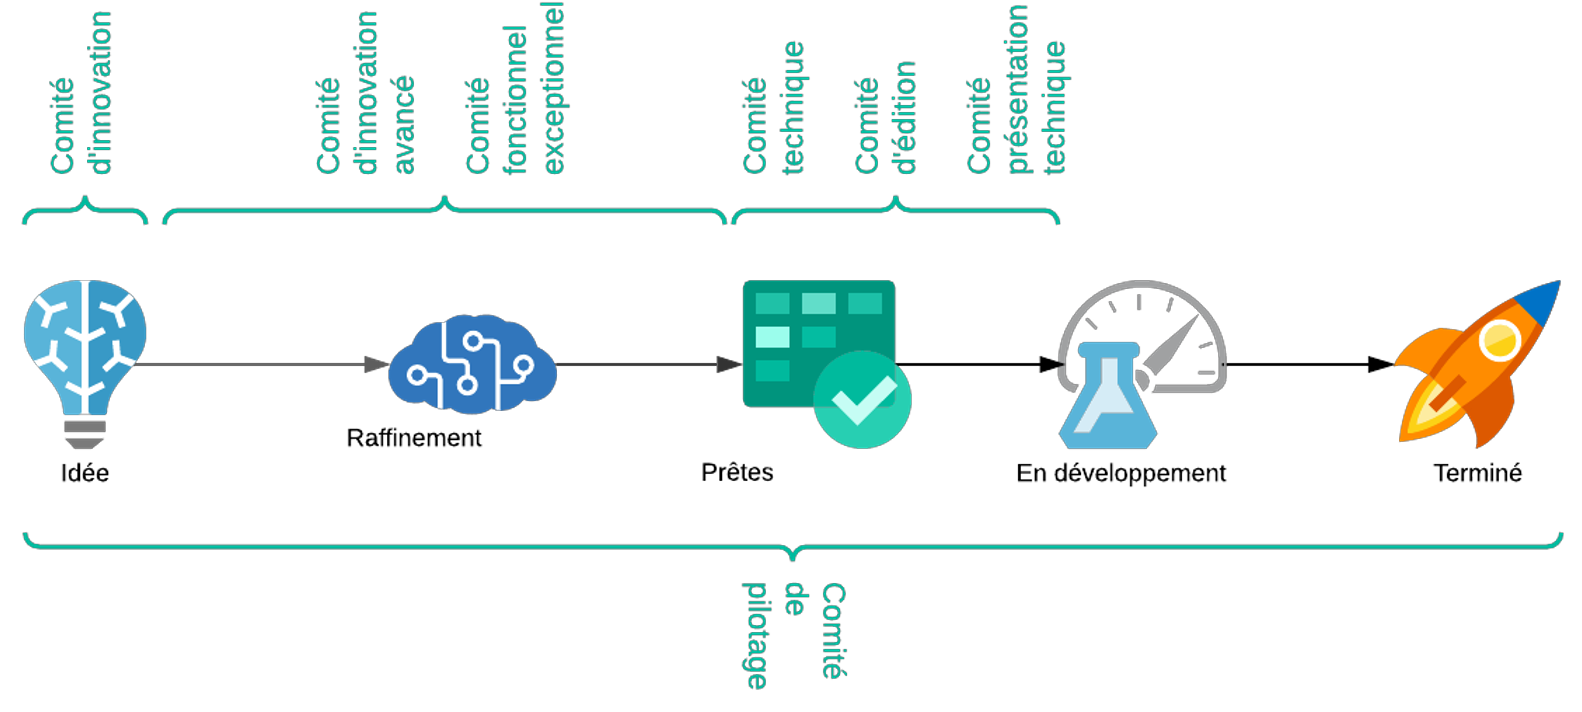
\includegraphics[width=\textwidth]{img/committees}
    \caption{La participation des différents comités au processus de traitement des idées d'innovation.}
    \label{fig:committees}
\end{figure}

Une édition représente le fruit de quatre mois de travail de développement, cependant, son élaboration ne s'arrête pas là. Elle englobe la mise en place et la planification des activités de communication (marketing), la formation des équipes support et commerce, la rédaction de manuels et de tutoriels destinés aux clients, ainsi que la préparation des prochaines éditions à venir.

\begin{longtblr}[
    caption={Les caractéristiques des différents comités.},
    label={tblr:character-committees}
    ]{
    hlines,vlines,
    rowspec={Q[m,font=\footnotesize\bfseries,gray9]*{7}{Q[m,font=\footnotesize]}}
    }
    {Nom du        \\ comité}       & {Récur-\\rence}   & Objectif          & Entrées & Sorties \\
    {Comité        \\ d'innovation} & {Hebdo-\\madaire} & {Première analyse                     \\ des idées exprimées                     \\ puis étude de l'intérêt \\ de chaque idée.} & {Liste des \\ idées} & {Idées clarifiées, \\ note par niveau \\ d'intérêt} \\
    {Comité        \\ d'innovation \\ avancé} & Mensuel & {Clarifier les \\ spécifications \\ fonctionnelles des \\ idées exprimées au \\ cours des comités \\ d'innovations.} & {Ordre du jour \\ des idées, déjà \\ analysées} & {Réponses aux \\ questions \\ à l'ordre du \\ jour, ajoutées \\ aux backlog} \\
    {Comité        \\ fonctionnel \\ exceptionnel} & {Excep-\\tionnel} & {Le PO sollicite une \\ partie prenante \\ identifiée, qui devrait \\ lui permettre de \\ lever un certain \\ nombre de questions \\ autour d'une \\ fonctionnalité.} & {Fonctionnalités, \\ déjà analysées \\ et comportant \\ toujours \\ des questions} & {Les réponses \\ sont ajoutées \\ aux \\ fonctionnalités} \\
    {Comité        \\ tech} & {En fonction \\ des items \\ en attente \\ de chiffrage \\ dans le \\ backlog. \\ Au moins \\ hebdo-\\madaire.} & {Une présentation \\ des items, validés \\ fonctionnellement, \\ pour faire ressortir \\ un macro-chiffrage, \\ réalisé par l'équipe \\ d'expert.} & {Fonctionnalités \\ prêtes du \\ backlog \\ produit} & {Macro-chiffrage \\ ou questions \\ fonctionnelles} \\
    {Comité        \\ pilotage} & {Bimestriel} & {Donner une vision \\ claire de l'avancement \\ du travail réalisé \\ pour les services \\ concernés.} & {Indicateur clé \\ de performance \\ à partager} & {Adaptations \\ à mettre en \\ œuvre} \\
    {Comité        \\ d'édition} & {Bimestriel} & {Établir une \\ constitution \\ d'édition à partir \\ des idées prêtes. \\ En déduire un \\ objectif d'édition \\ permettant de \\ fédérer autour \\ d'une réalisation.} & {Fonctionnalités \\ prêtes, analyse du \\ temps disponible \\ faite à partir \\ des paramètres \\ vélocité / nombre \\ de demandes \\ courantes / dette \\ technique \dots
    } & {Liste des \\ composants \\ d'édition, \\ objectif \\ d'édition} \\
    {Comité        \\ présentation \\ technique /\\ Kickoff \\ Edition} & {En début \\ d'édition} & {Une présentation des \\ items embarqués dans \\ l'édition, ainsi qu'un \\ focus sur l'objectif \\ d'édition.} & {L'objectif, \\ le contenu \\ d'édition} & {Le retour \\ de l'équipe \\ sur le contenu \\ et l'objectif}
\end{longtblr}

\section{Méthodologie Agile}\label{sec:agile}

L'équipe de développement de la géolocalisation de SuiviDeFlotte -- comme les autres équipes de développement de l'entreprise -- travaille selon la méthodologie agile SCRUM. Cette méthodologie est une approche de gestion de projet qui met l'accent sur la flexibilité, la collaboration et la livraison continue. Elle est largement utilisée dans le développement de logiciels et peut également être appliquée à d'autres domaines. SCRUM divise un projet en cycles appelés \foreignquote{french}{itérations} ou \foreignquote{french}{sprints} de courte durée, généralement de deux à quatre semaines, pendant lesquels une partie du travail est accomplie et livrée.

Les termes clés de la méthodologie SCRUM sont énumérés ci-dessous et illustrés dans la Figure~\ref{fig:agile}.

\begin{description}
    \item[Product Owner (Propriétaire du Produit)] La personne responsable de définir et de prioriser les éléments du produit à développer. Le Propriétaire du Produit représente les besoins des utilisateurs et des parties prenantes.
    \item[Scrum Master (Maître de Scrum)] Le facilitateur du processus SCRUM. Le Scrum Master s'assure que l'équipe suit les principes SCRUM, élimine les obstacles et favorise un environnement de travail efficace.
    \item[Équipe de Développement] Le groupe de professionnels chargé de concevoir, développer, tester et livrer les éléments du produit à la fin de chaque sprint.
    \item[User Story (Histoire Utilisateur)] Une Histoire Utilisateur est une courte description d'une fonctionnalité ou d'un aspect du produit, racontée du point de vue de l'utilisateur. Elle suit généralement le format \foreignquote{french}{En tant que [utilisateur], je veux [action] afin de [objectif]}. Les Histoires Utilisateurs sont des éléments du Carnet de Produit et aident à définir les fonctionnalités du produit du point de vue de l'utilisateur.
    \item[Story Point (Point d'Histoire)] Le Point d'Histoire est une unité relative utilisée pour estimer la complexité, l'effort et la taille des Histoires Utilisateurs ou des tâches de développement. Il n'a pas de valeur absolue, mais il sert à comparer la difficulté relative entre différentes Histoires Utilisateurs. Les équipes de développement attribuent des points d'histoire lors des estimations, ce qui les aide à planifier la quantité de travail qu'elles peuvent accomplir dans un sprint donné.
    \item[Epic (Épique)] Un Épic est une unité de travail plus large que les Histoires Utilisateurs individuelles. Il représente généralement un ensemble de fonctionnalités, de tâches ou de travaux qui sont trop importants pour être traités dans un seul sprint. Les Épics sont souvent des objectifs à long terme qui sont décomposés en Histoires Utilisateurs plus petites et gérables. Ils aident à organiser et à structurer le développement du produit en regroupant des éléments liés autour d'un thème ou d'un objectif commun. Les Épics sont inclus dans le Carnet de Produit et sont priorisés en fonction de leur valeur pour l'utilisateur et du contexte global du projet.
\end{description}

SCRUM encourage la transparence, l'adaptabilité et la collaboration continue entre les membres de l'équipe et les parties prenantes, ce qui permet de s'adapter aux changements et de fournir rapidement de la valeur tout au long du projet.

\begin{figure}[ht]
    \centering
    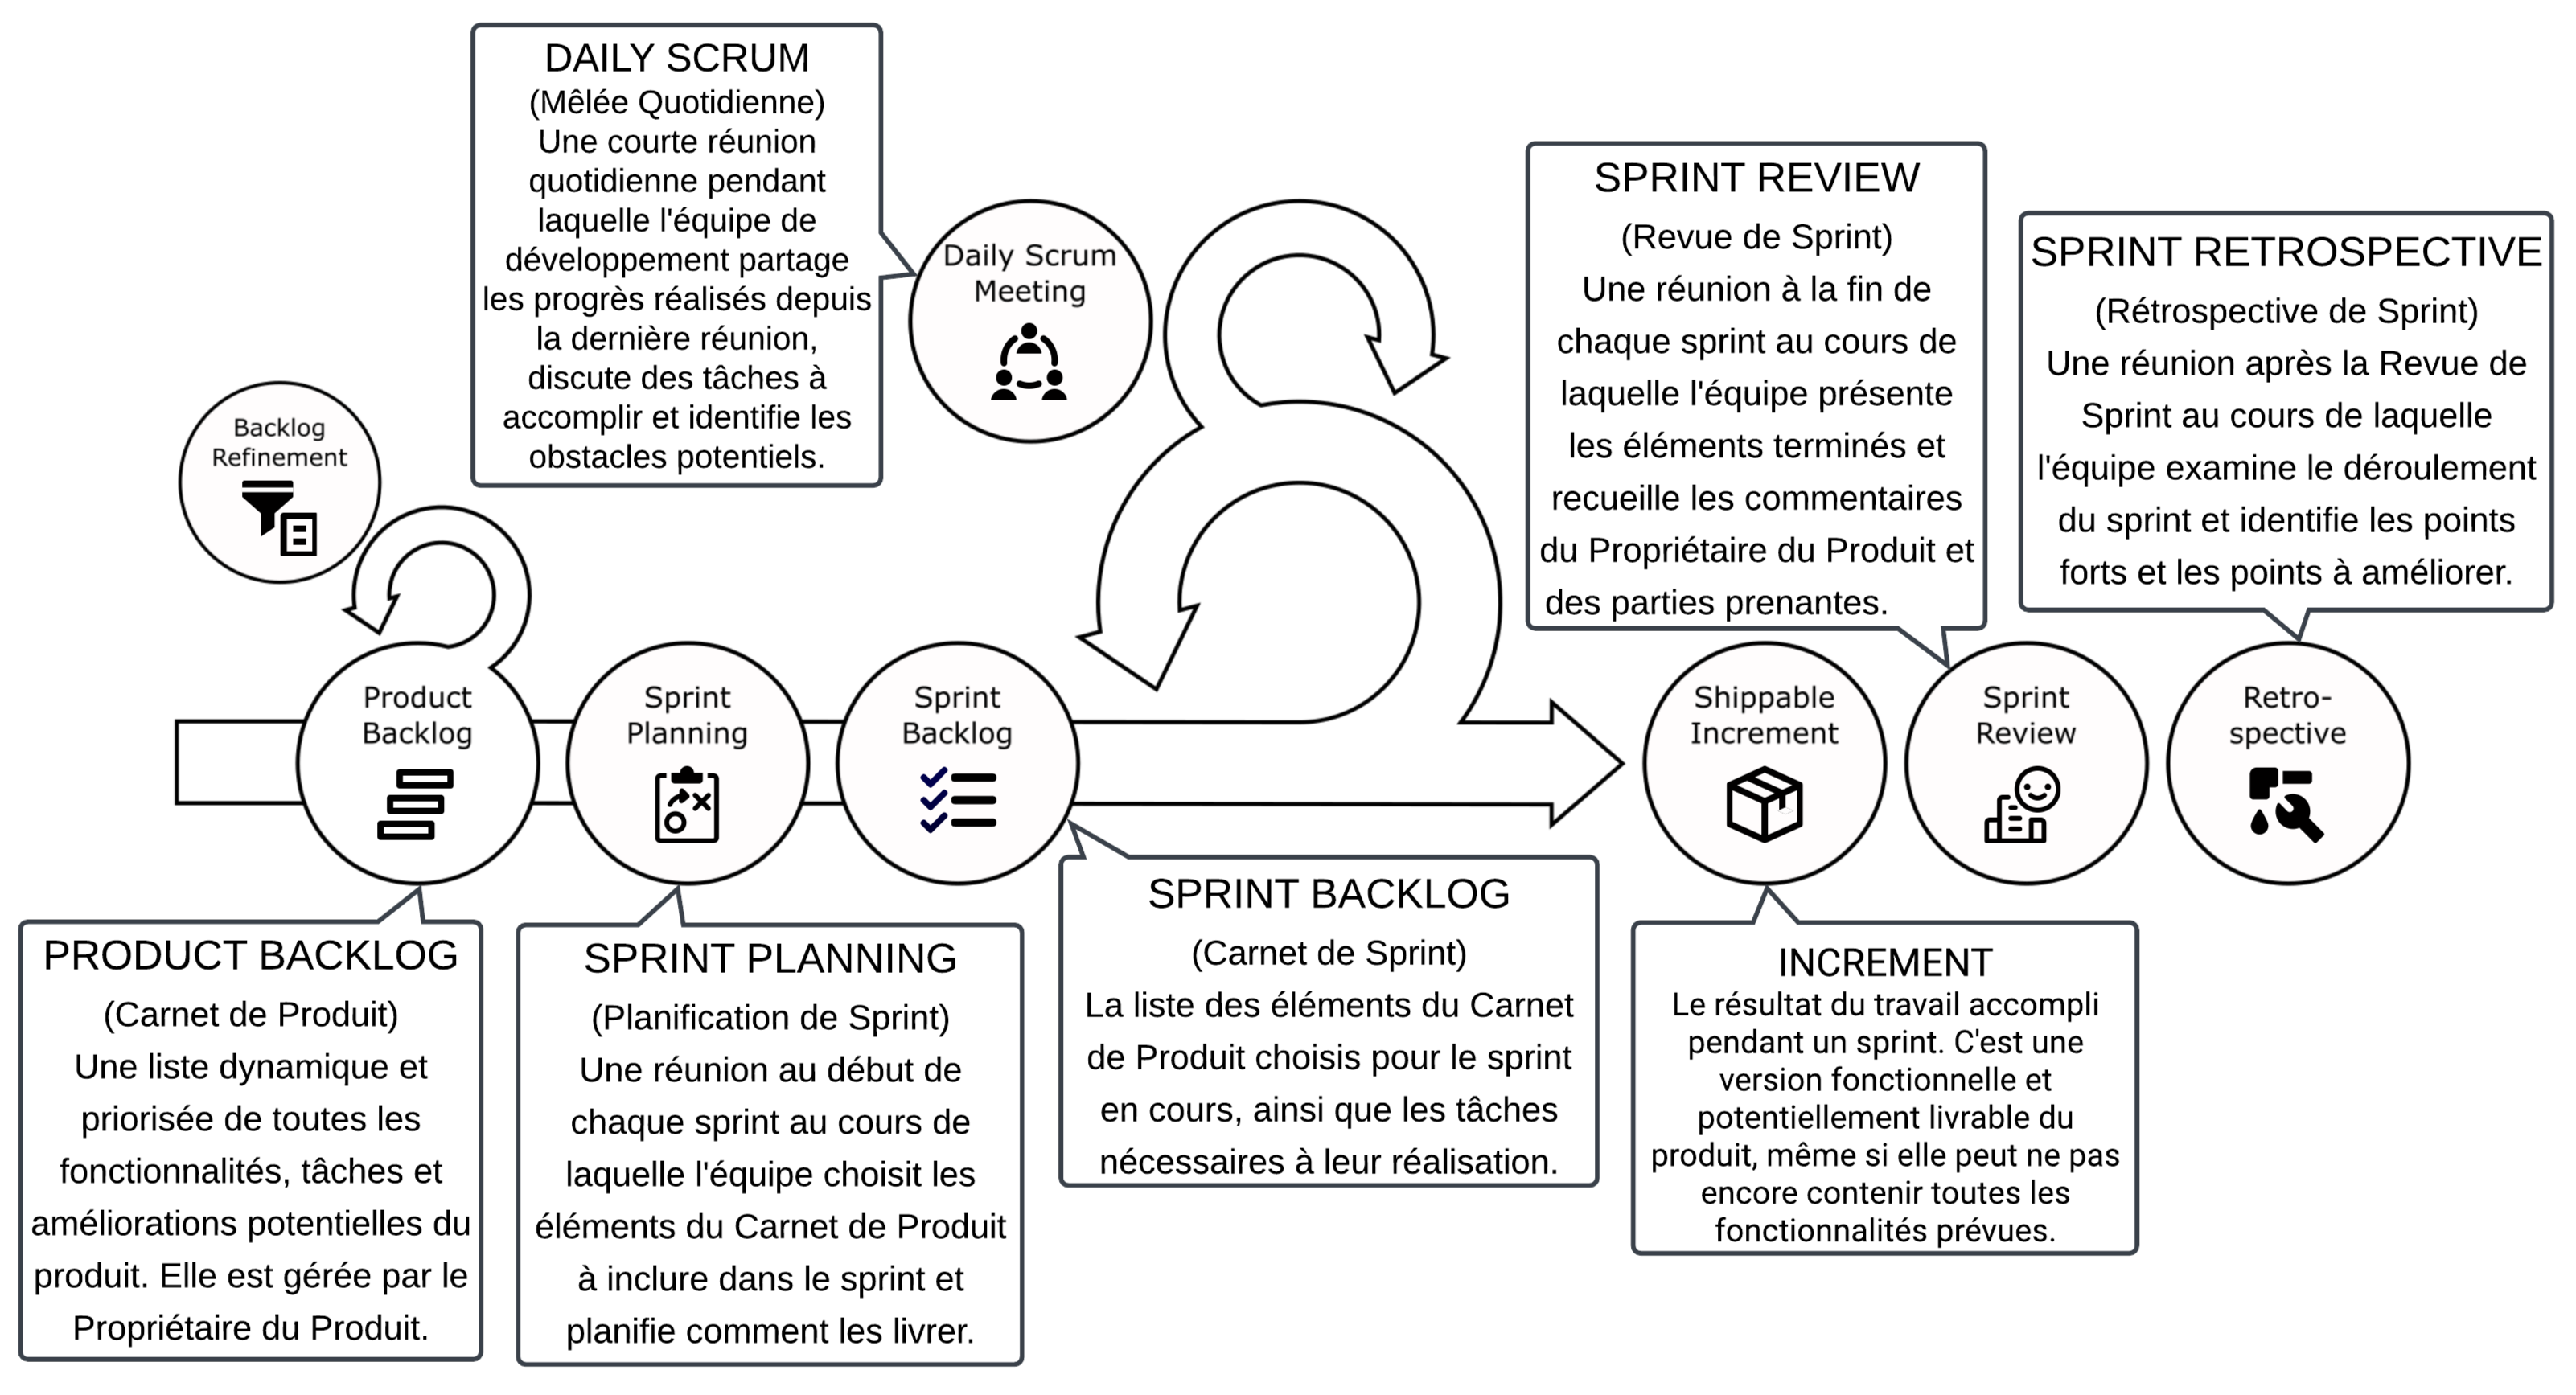
\includegraphics[width=\textwidth]{img/agile-02}
    \caption{Cérémonies SCRUM.}
    \label{fig:agile}
\end{figure}

Dans l'équipe Géoloc, le processus suit un calendrier de sprints de deux semaines (Figure~\ref{fig:sprint}). Chaque cycle commence par un ensemble de réunions clés qui ont lieu tous les deuxièmes mardis. Cette journée englobe la Revue de Sprint, la Rétrospective de Sprint et la Planification de Sprint. Lors de la Revue de Sprint, les éléments achevés sont présentés au Propriétaire du Produit et aux parties prenantes, les retours sont recueillis et les priorités sont ajustées si nécessaire. La Rétrospective de Sprint offre l'opportunité à l'équipe de réfléchir aux succès et d'identifier les domaines à améliorer, favorisant une culture d'amélioration continue. Ensuite, la Planification de Sprint implique la sélection des Histoires Utilisateurs du Carnet de Produit à inclure dans le sprint à venir, en tenant compte de leur complexité et de leur priorité. Pour l'estimation de la complexité des tâches, des Points d'Histoire basés sur la séquence de Fibonacci (1, 2, 3, 5, 8, 13) sont utilisés. Cette approche aide à attribuer des valeurs relatives à différentes tâches et assure une évaluation cohérente de la charge de travail.

À la fin de chaque sprint, les nouveaux incréments sont également mis en production. Grâce à l'approche Agile et à la fréquence des mises en production, les modifications apportées à l'application sont rapidement portées à la connaissance de l'utilisateur.

Chaque jour ouvrable débute par une Mêlée Quotidienne de 15 minutes, au cours de laquelle les progrès depuis la dernière réunion sont passés en revue, les tâches sont discutées et les obstacles potentiels sont identifiés. Ces réunions se déroulent généralement en ligne via Google Meet pour accueillir les collègues travaillant à distance et garantir la participation de tous les membres de l'équipe, peu importe leur emplacement. Par contre, pour maintenir la communication et la cohésion de l'équipe, les réunions du mardi de chaque deuxième semaine sont des réunions en personne. Cette pratique encourage les échanges directs, la collaboration étroite entre les membres de l'équipe et facilite la résolution rapide de tout problème ou obstacle pouvant survenir.

\begin{figure}[ht]
    \centering
    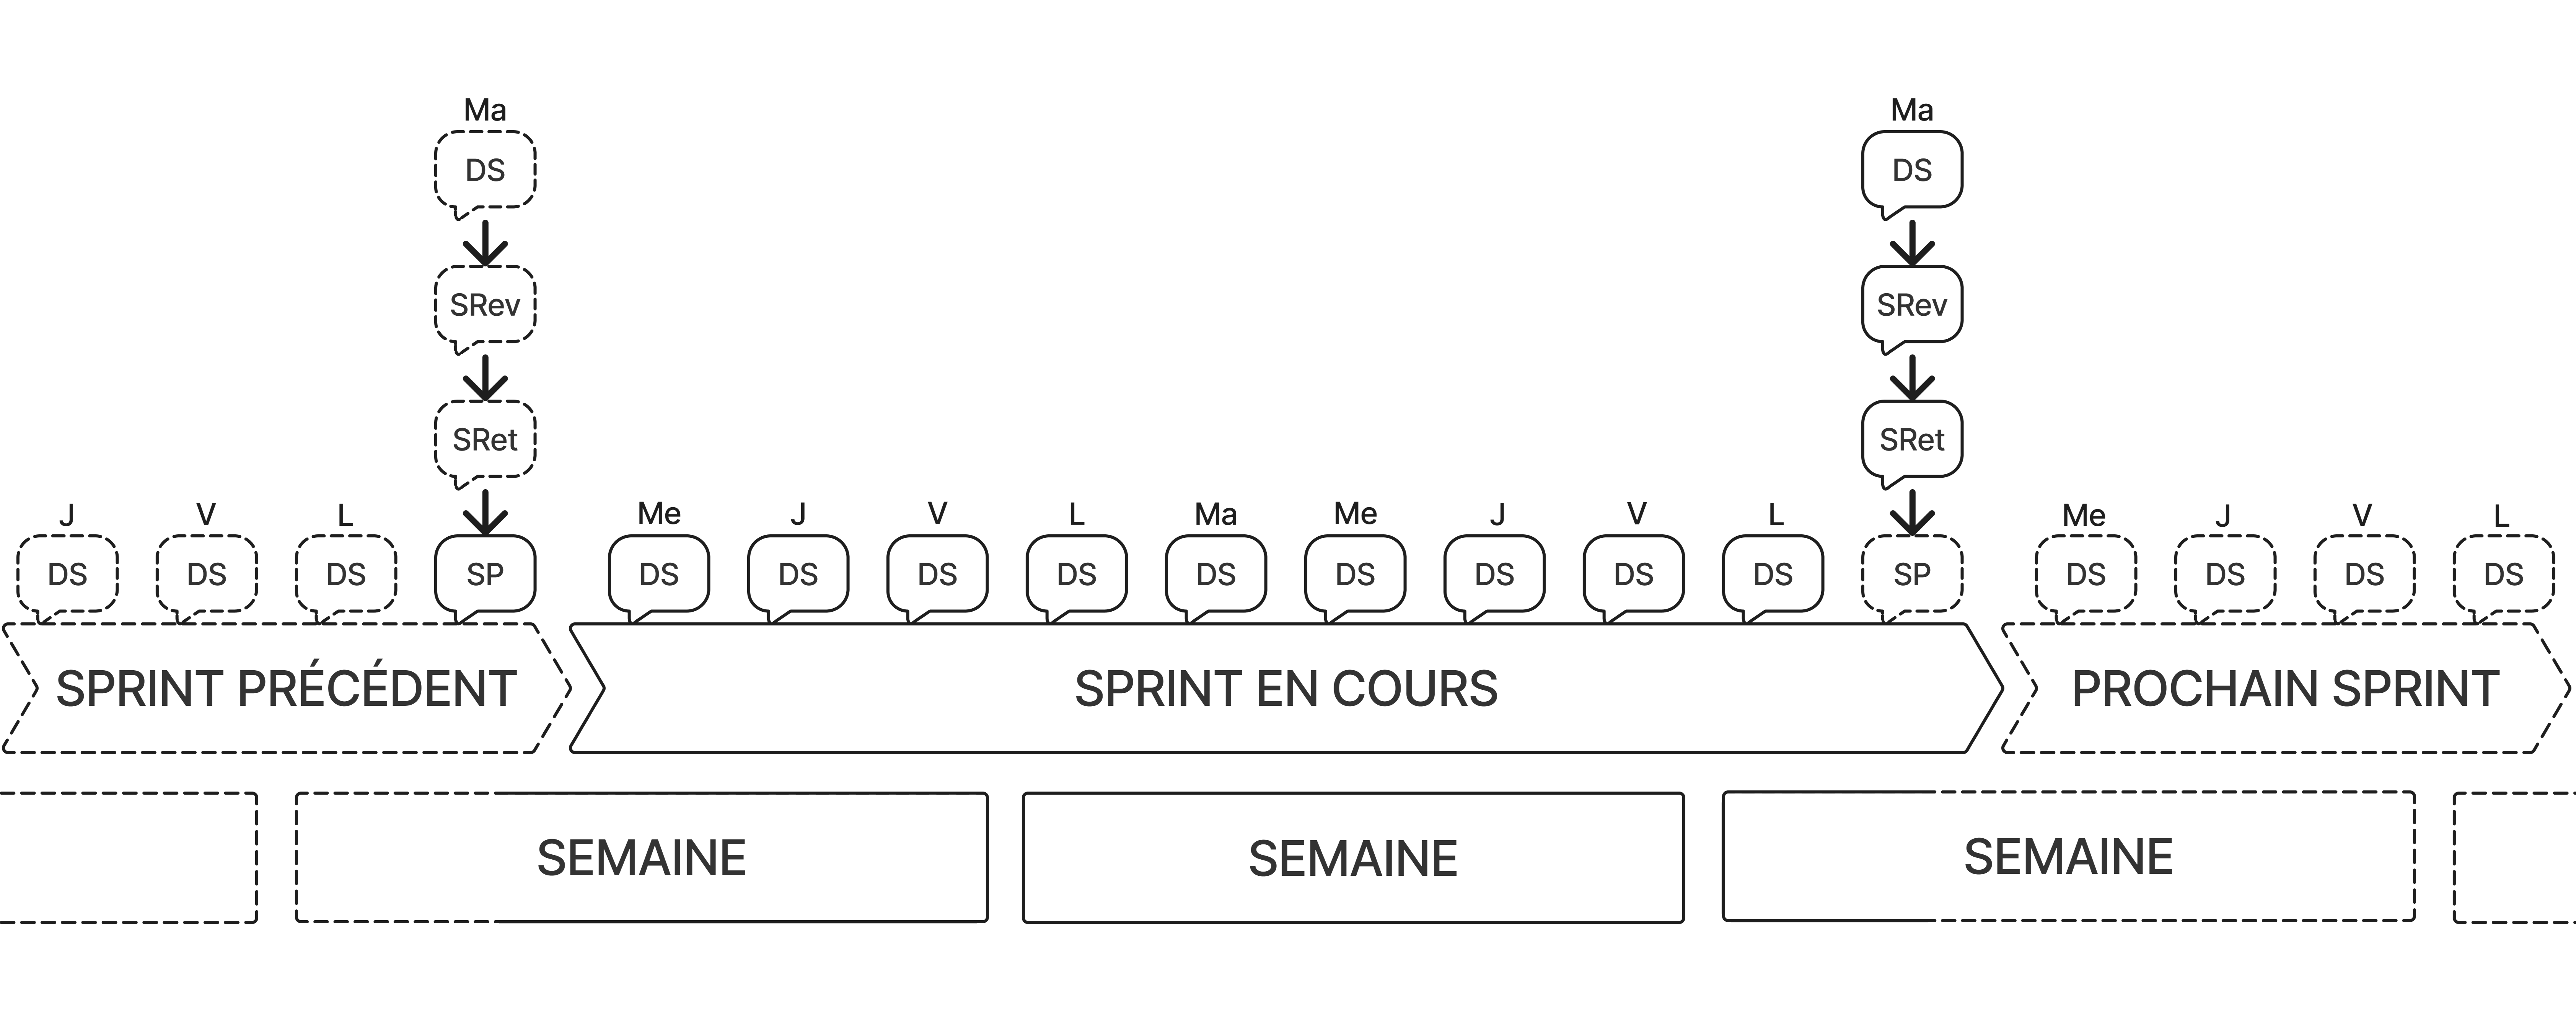
\includegraphics[width=\textwidth]{img/sprint04}
    \caption{Programme des sprints chez SuiviDeFlotte. Légende : L, Ma, Me, J, V -- jours de la semaine ; DS -- Daily Scrum ; SRev -- Sprint Review ; Sret -- Sprint Retrospective ; SP -- Sprint Planning ; ligne pointillée -- Sprint précédent ou suivant ; ligne continue -- Sprint en cours.}
    \label{fig:sprint}
\end{figure}

Actuellement, les rôles du Propriétaire du Produit et du Maître de Scrum ont été temporairement fusionnés en une seule personne. Cette configuration permet au Propriétaire du Produit de gérer les responsabilités du projet tout en facilitant le processus SCRUM, en maintenant une communication fluide avec l'équipe de développement.

En complément des cycles de deux semaines des Sprints, l'opération de l'entreprise comprend également un cycle plus long. En effet, comme je l'ai mentionné dans l'introduction de ce chapitre, l'entreprise publie une nouvelle version, appelée nouvelle Edition, de ses services en ligne tous les quatre mois, soit trois fois par an. Cela implique qu'il y a environ huit sprints pour que les développeurs puissent concevoir les nouvelles fonctionnalités des nouvelles éditions.

La Figure~\ref{fig:committees-and-scrum} résume les relations entre les comités et le processus des sprints. Comme on peut le voir, les tickets du Carnet de produit proviennent du Comité d'innovation, du Comité d'innovation avancée, du Comité fonctionnel exceptionnel, du Comité d'édition et du Comité d'innovation technique. Ensuite, le Comité d'édition sélectionne les tickets pour la prochaine Edition et le Comité de présentation technique les présente à l'équipe de développeurs. Une autre source de tickets dans le Backlog de Produit est l'équipe de support qui crée des tickets de bogues. Le traitement des bogues est illustré par la Figure~\ref{fig:treatment-of-bugs}. La section suivante explique comment ces tickets sont traités dans un outil appelé Jira.

\begin{figure}[ht]
    \centering
    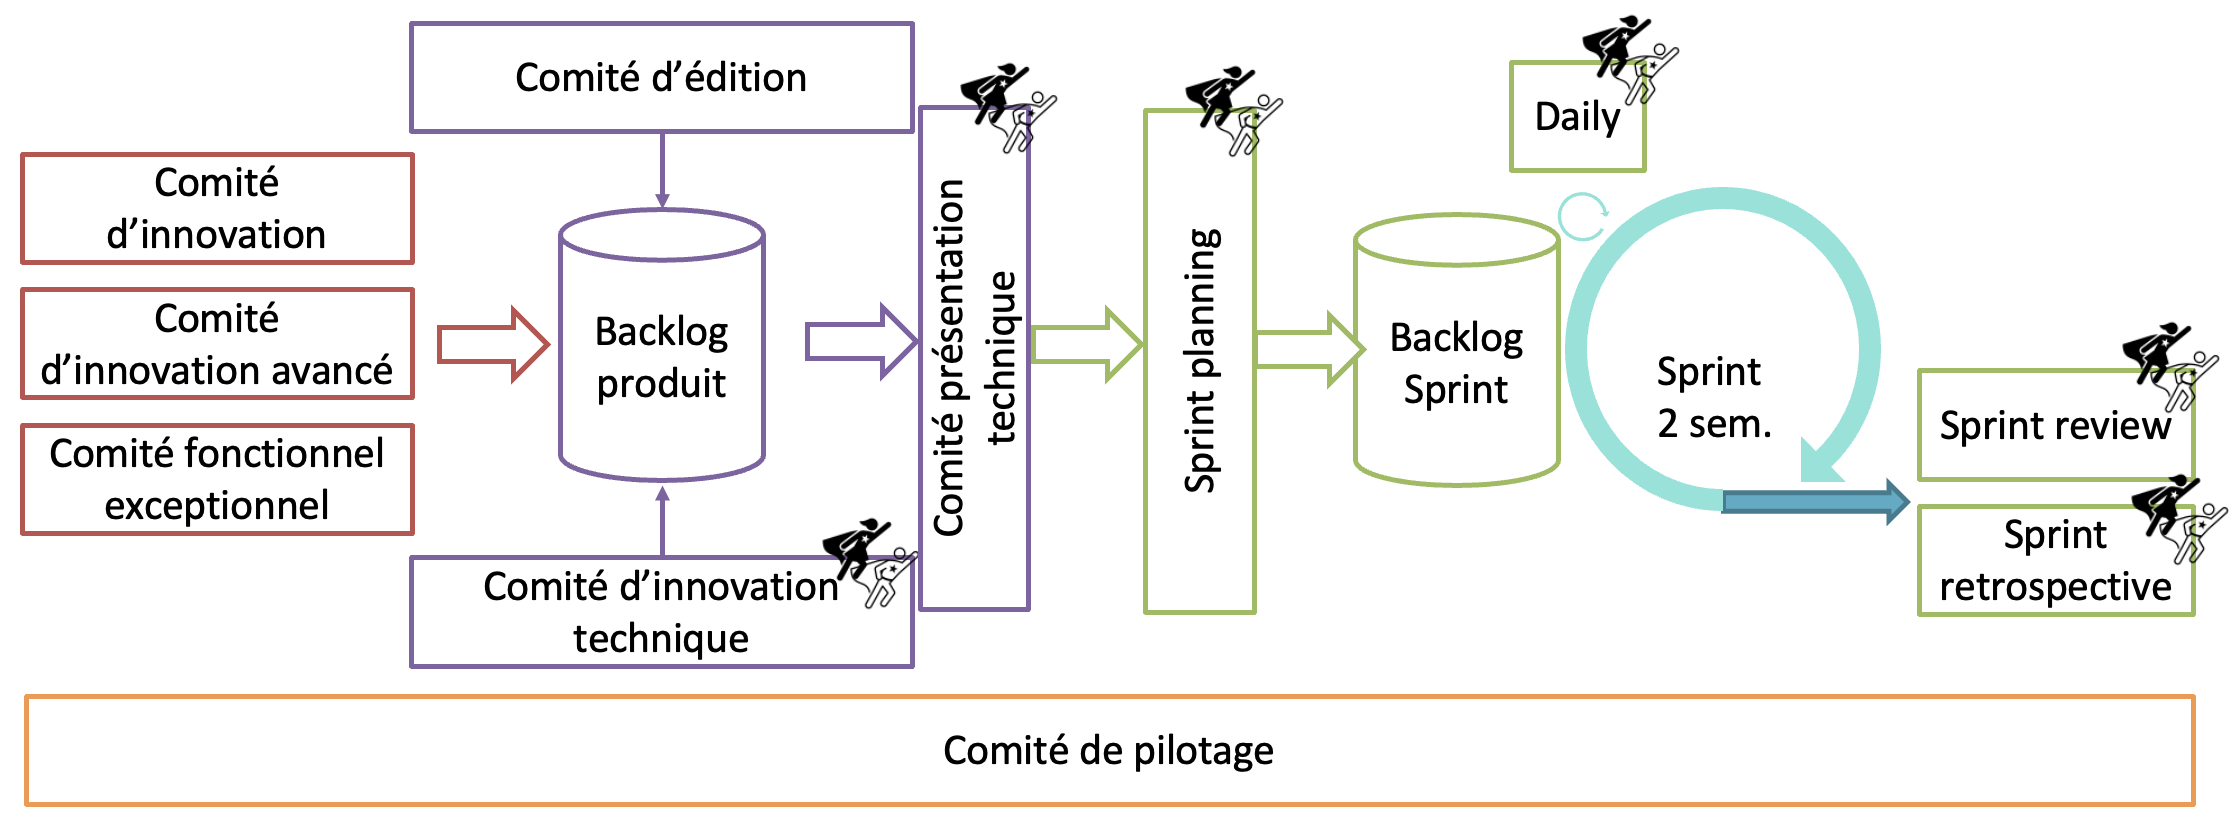
\includegraphics[width=\textwidth]{img/committees-and-scrum}
    \caption{Résumé des relations entre les comités et le processus des sprints.}
    \label{fig:committees-and-scrum}
\end{figure}

\begin{figure}[ht]
    \centering
    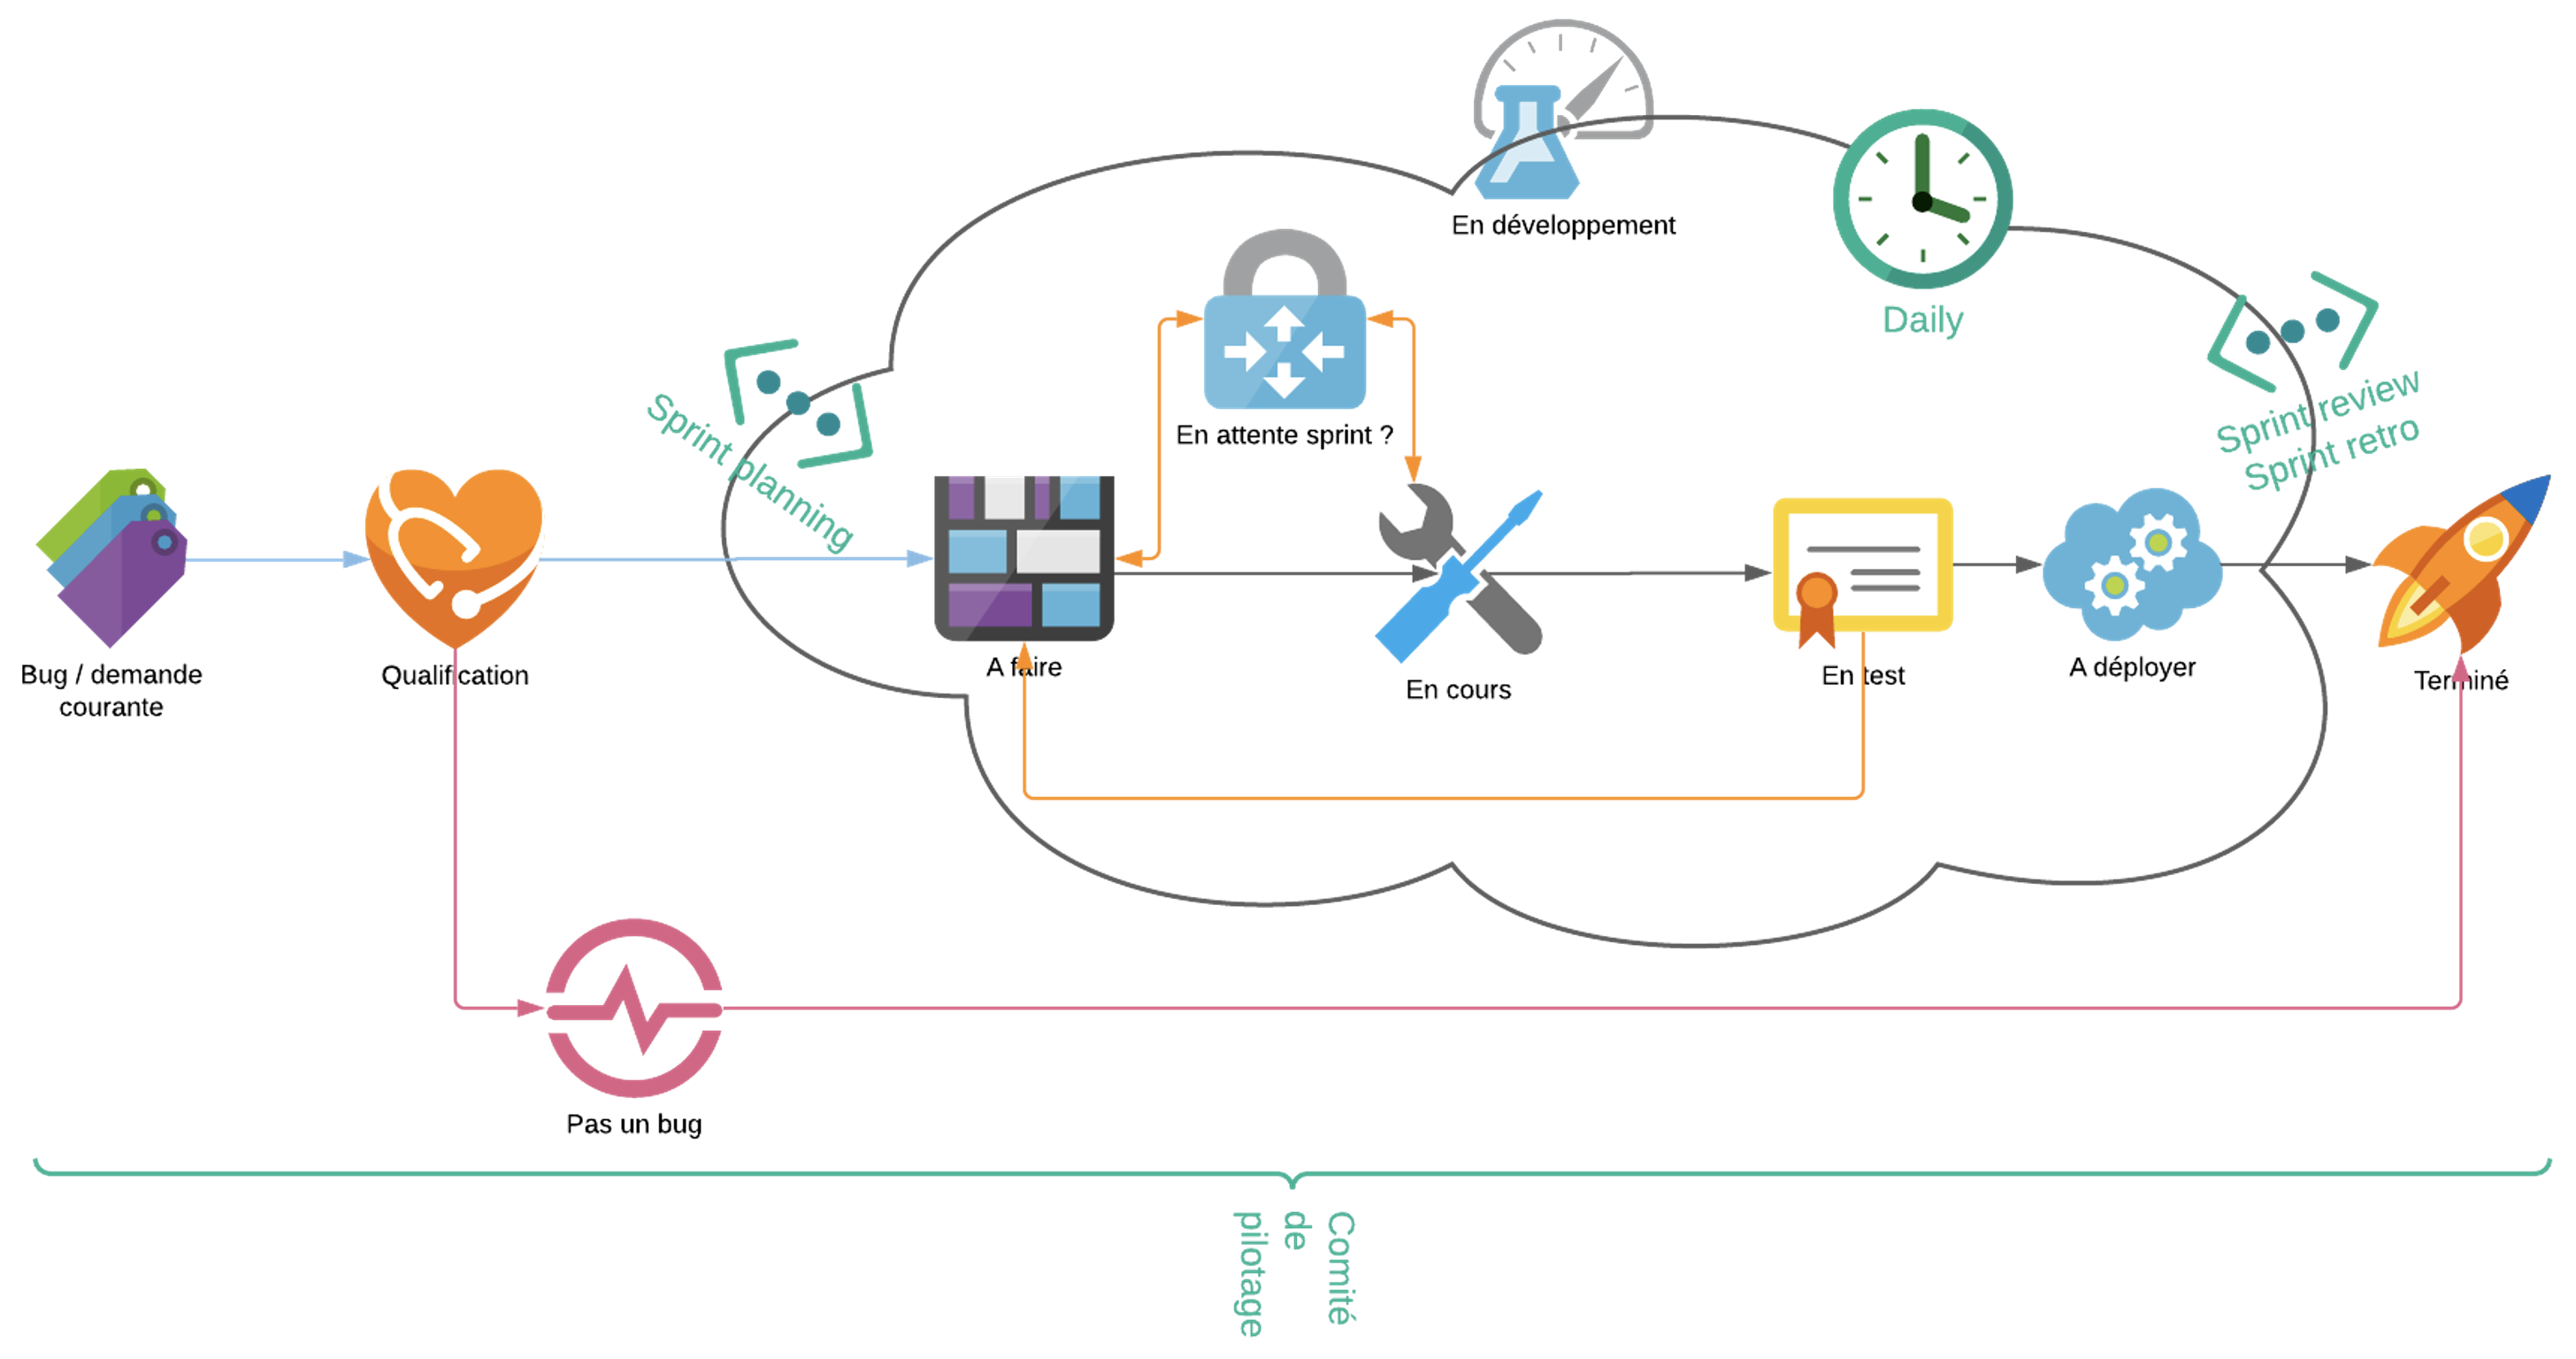
\includegraphics[width=\textwidth]{img/treatment-of-bugs}
    \caption{Diagramme d'activité du traitement des bugs.}
    \label{fig:treatment-of-bugs}
\end{figure}
\section[Jira : L'outil essentiel pour la gestion de projet]{Jira : L'outil essentiel pour la gestion quotidienne de projet}\label{sec:jira}

Au sein de l'entreprise, les équipes SCRUM se servent de Jira afin de consigner et de suivre tous les aspects de leur travail.

Jira est un outil essentiel pour les équipes SCRUM car il facilite la gestion complète du processus de développement agile. Il permet aux équipes de collaborer de manière efficace et de suivre chaque étape du cycle de vie du projet. Avec Jira, les équipes SCRUM peuvent créer, organiser et hiérarchiser leur Carnet de Produit en ajoutant des Histoires Utilisateurs, des tâches, des Épics et des bugs.

L'outil facilite la planification des sprints en permettant aux équipes de sélectionner les éléments du Carnet de Produit à inclure dans chaque itération. Les équipes peuvent estimer la complexité des tâches à l'aide de Story Points et suivre leur progression au fil du temps.

Les fonctionnalités de suivi des tâches et des problèmes dans Jira aident les équipes à gérer leur travail quotidien. Chaque membre de l'équipe peut mettre à jour l'état de ses tâches, signaler les obstacles et collaborer de manière transparente avec les autres membres de l'équipe.

Les réunions SCRUM telles que la Mêlée Quotidienne, la Revue de Sprint et la Rétrospective de Sprint peuvent être orchestrées efficacement grâce à Jira. L'outil permet de suivre les progrès, de partager les résultats et de documenter les réflexions pour chaque itération.

Les flux de travail (workflows) dans Jira constituent un mécanisme central pour orchestrer et suivre le déroulement des tâches et des projets. Ces flux définissent les étapes spécifiques à suivre pour qu'une tâche ou un problème progresse, de sa création à son achèvement. Les équipes peuvent personnaliser ces flux pour refléter leurs processus uniques, en définissant les transitions entre les étapes et en assignant des responsabilités à différents membres de l'équipe. Les flux de travail de Jira contribuent à maintenir la transparence, à améliorer l'efficacité et à garantir que toutes les parties prenantes restent informées de l'avancement du travail. Grâce à cette fonctionnalité, les équipes peuvent gérer avec agilité et précision les tâches, tout en favorisant une collaboration fluide et une visibilité accrue sur les projets.

Chez SuiviDeFlotte, le diagramme d'activité présenté dans les Annexes, dans la Figure~\ref{fig:lifecycle-of-incoming-ideas} (page~\pageref{fig:lifecycle-of-incoming-ideas}) est la base du flux de travail dans Jira. La partie supérieure gauche du diagramme illustre à nouveau le traitement des idées novatrices par les différents comités. En revanche, la partie supérieure droite présente le traitement des bogues (demandes courantes) qui proviennent de l'équipe de support. Ensuite, le propriétaire du produit sélectionne les tickets pour le prochain sprint à partir de l'ensemble des tickets prêts. Ce diagramme contient les étapes suivantes, qui sont utilisées comme étapes du flux de travail dans Jira : en raffinement, à faire, en cours, en test, à déployer, terminé, abandonné.

Un autre diagramme d'activité montre plus en détail le traitement des bogues (Annexes, Figure~\ref{fig:lifecycle-of-bugs}, page~\pageref{fig:lifecycle-of-bugs}). À partir de ce diagramme, nous pouvons ajouter quelques étapes supplémentaires à la liste des étapes du flux de travail : en attente, en attente support.

Le diagramme de flux de travail qui en résulte et qui est actuellement utilisé est présenté à la Figure~\ref{fig:workflow}.

\begin{figure}[ht]
    \centering
    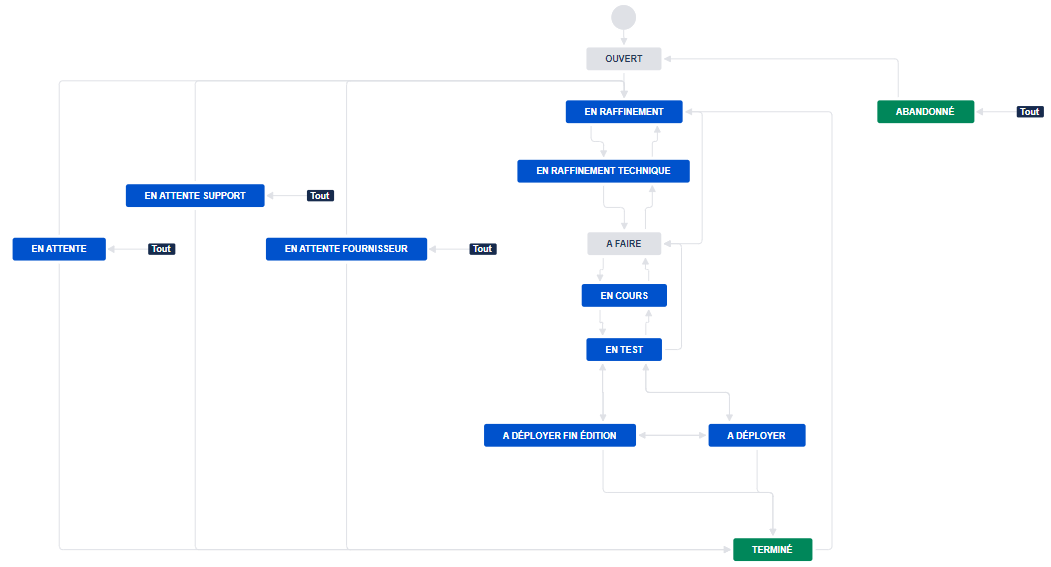
\includegraphics[width=\textwidth]{img/workflow-sdfn}
    \caption{Le flux de travail utilisé dans Jira chez SuiviDeFlotte.}
    \label{fig:workflow}
\end{figure}

Dans les Annexes, la Figure~\ref{fig:product-backlog} (page~\pageref{fig:product-backlog}) et la Figure~\ref{fig:sprint-backlog} (page~\pageref{fig:sprint-backlog}) présentent un exemple de Backlog de produit et de Backlog de sprint sous forme de tableau Kanban, et la Figure~\ref{fig:ticket} (page~\pageref{fig:ticket}) donne un exemple d'un ticket.

\section{Versioning avec Git et GitLab}\label{sec:versioning-git-gitlab}

Dans l'entreprise, les équipes de développement utilisent Git pour la gestion des versions et GitLab pour gérer le processus de développement.

Git est un système de gestion de version décentralisé largement utilisé dans le développement de logiciels. Il permet aux équipes de collaborer efficacement sur des projets en suivant les modifications apportées aux fichiers au fil du temps. Grâce à Git, les développeurs peuvent créer des branches pour travailler sur des fonctionnalités spécifiques ou des corrections de bugs sans perturber le code principal. Les commits, qui représentent des enregistrements de changements, sont la pierre angulaire de Git, permettant de garder une trace claire de l'évolution du code.

GitLab, quant à lui, est une plateforme de gestion de développement logiciel basée sur Git. Elle offre un environnement complet pour le cycle de vie du développement, de la planification à la surveillance. GitLab permet aux équipes de suivre les problèmes, de planifier les sprints, de gérer les demandes d'extraction et de créer des pipelines d'intégration continue pour automatiser les tests et le déploiement. En regroupant toutes ces fonctionnalités au même endroit, GitLab facilite la collaboration entre les membres de l'équipe et permet une gestion transparente et efficace des projets de développement.

Parmi ces nombreuses fonctionnalités, les équipes de DevOps et de développement n'utilisent cependant pas les fonctionnalités de gestion de projet et d'intégration continue/de livraison continue de GitLab, puisqu'elles utilisent Jira (comme nous l'avons vu dans la section précédente) et TeamCity (comme nous le verrons dans la section suivante) à ces fins. GitLab est donc principalement utilisé comme un hébergeur de dépôt de code et un outil de révision de code avec des fonctionnalités telles que les demandes de fusion (merge request).

La Figure~\ref{fig:versioning-and-environments} illustre les principes du versioning et les différents environnements utilisés pour héberger les différentes versions du code. Le tableau Y apporte quelques compléments d'information.

\begin{sidewaysfigure}
    \centering
    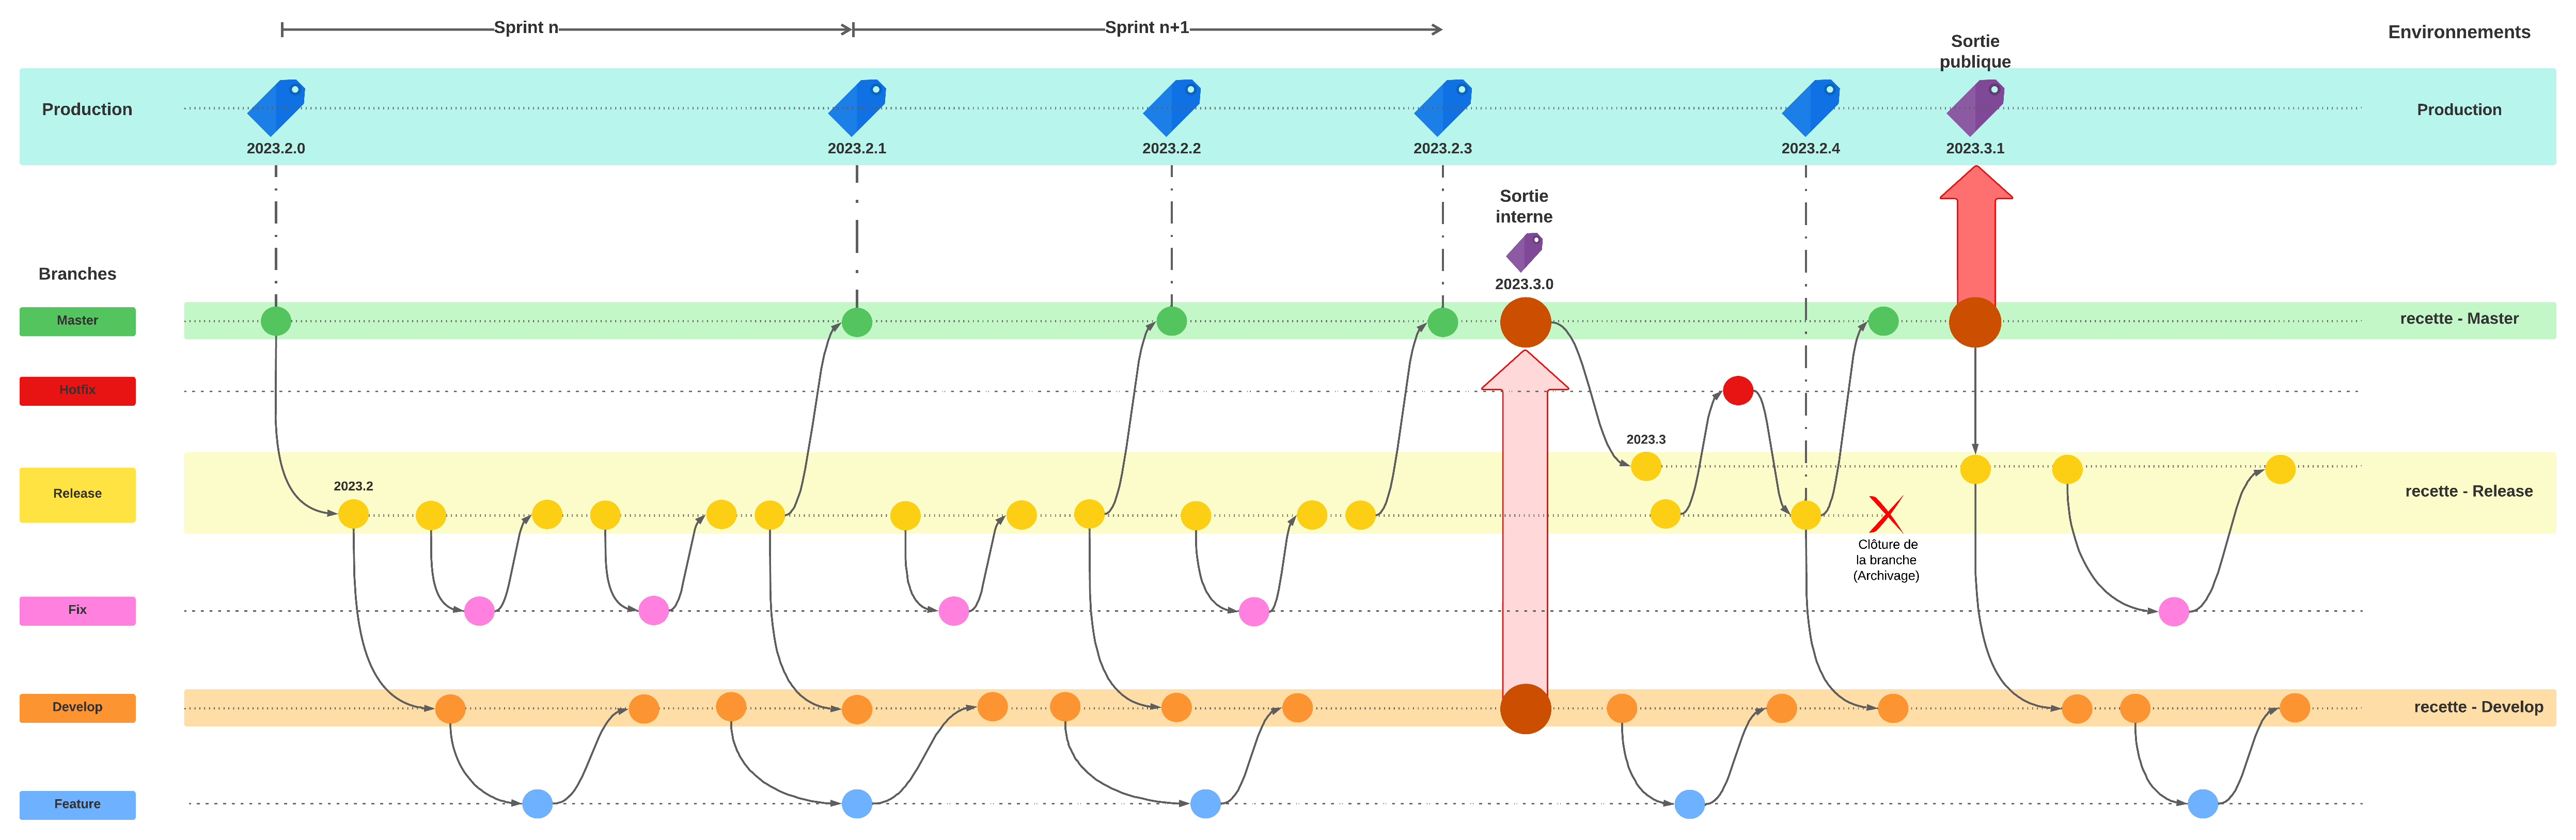
\includegraphics[width=\textwidth]{img/versioning-and-environments}
    \caption{Le schéma du versioning et des environnements.}
    \label{fig:versioning-and-environments}
\end{sidewaysfigure}

\begin{longtblr}[
    caption={Les caractéristiques des différents environnements.},
    label={tblr:environments}
    ]{
    hlines,vlines,
    rowspec={Q[m,font=\footnotesize\bfseries,gray9]*{5}{Q[m,font=\footnotesize]}}
    }
    Environnement    & {Pour quels                       \\ services} & Branches & {Type de \\ comits} & {Déploiement \\ TeamCity} \\
    {Dev pour chaque                                     \\ développeur} & Développeur & {Développeur \\ sandbox} &  & -- \\
    recette-develop  & {Le PO vérifie                    \\ les fonction-\\nalités}                                & develop             & feat                                                         & Auto                                                                      \\
    recette-releases & {Le PO vérifie                    \\ les corrections}                                    & releases/édition    & fix                                                          & Auto                                                                      \\
    recette-master   & {Autres                           \\ services                    \\ pour test \\ (direction, \\ marketing, \\ commerce \\ \dots)} & master              & {(env juste \\ avant la prod, \\ préproduction)}                     & {Manuel, \\ section master \\ dans TeamCity, \\ demande via \\ ticket MEP \\ à DevOps}     \\
    production       &                & tag & {Commit en \\ production \\ avec tag \\ \{numéro-édtion\}.\\\{numéro-increment\}} & {Manuel, \\ section \\ production \\ dans TeamCity, \\ demande via \\ ticket MEP \\ à DevOps}
\end{longtblr}

\section{CI/CD : Intégration Continue et Déploiement Continu}\label{sec:ci-cd}

\section{Cycle de vie d'une nouvelle évolution}\label{sec:cycle-de-vie}
\chapter{Cahier des charges}\label{ch:cahier}

L'année dernière, la société constatait sur ses solutions une véritable disparité de méthodologies d'intégration pour les documents. Chaque fonctionnalité intégrait les documents de manière différente, ce qui les amenait à constater qu'il était alors compliqué de répondre rapidement à ce type de besoins.

De plus, elle avait d'une part des demandes d'importation de nouveaux fournisseurs de carburant, mais également d'autre part la création du poste de CSM (Customer Success Manager). En outre, suite à un besoin exprimé par l'un de ses grands clients, il y avait de plus en plus de besoins pour intégrer rapidement et efficacement de nouvelles typologies de documents.

Basé sur ce constat, l'entreprise a donc décidé qu'il était nécessaire de construire un outil permettant de répondre à ces besoins : le Pipeline documentaire.

Son projet était qu'à terme, cet outil leur permettrait de généraliser l'intégration des fichiers dans leur solution. Il serait donc le point d'entrée central pour tous les documents entrant dans chacun de leurs logiciels. L'ajout d'une nouvelle typologie de document serait simple et se ferait, pour la partie intégration du moins, principalement à travers le paramétrage.

La section suivante montre comment le propriétaire du produit a exprimé les besoins concernant le Pipeline documentaire.

\section{Expression des besoins}

\subsection{Concepts généraux}

Dans sa conception, ce nouvel outil devra être le plus détaché possible du reste de l'ensemble applicatif, afin d'être ensuite mis à disposition et utilisé par l'ensemble de nos logiciels, de manière simple et intégrée. Dans cette optique, l'outil devra donc être conçu pour être notre première \foreignquote{french}{Machine}, concept abordé lors de notre étude de la refonte globale, qui est donc un outil logiciel mis à disposition de l'ensemble des autres applications, mais qui reste complètement autonome.

\subsection{Composition de l'outil}

\subsubsection{Déclencheurs}

Le concept de déclencheur devra faire partie intégrante de la conception de l'outil, en suivant toujours les mêmes règles et en permettant de déclencher une intégration. Lorsqu'un déclencheur est \foreignquote{french}{appelé}, il lancera l'intégration complète. Celui-ci fournira au guide toutes les informations nécessaires ainsi que le ou les fichiers à intégrer. Cependant, chaque déclencheur sera indépendant et répondra à une intégration spécifique. Un certain nombre de déclencheurs ont été identifiés dans le schéma architectural (Figure~\ref{fig:architectural-schema}). Cependant, cette liste n'est pas exhaustive.

\subsubsection{Guide}

Dans notre outil, le guide sera le point central de l'intégration. Son rôle consistera à charger la configuration adéquate afin de réaliser l'intégration, puis à faire passer le ou les fichiers à travers la chaîne d'intégration, en fonction de la configuration préalablement mise en œuvre. En fin de compte, le guide aura pour objectif de piloter l'intégration complète du fichier, c'est-à-dire de s'assurer de son bon parcours à travers la chaîne d'intégration.


\subsubsection{Configurations}

Les fichiers de configuration devront être créés pour déclarer tout nouvel import. Chaque fichier de configuration aura un format informatique, mais restera lisible par un développeur (json, yml, etc.). Ces fichiers de configuration permettront, pour chaque type d'import, de définir ses spécificités et ainsi de déterminer chaque étape de l'import. Les principales informations incluses dans ces fichiers seront les suivantes :

\begin{itemize}
    \item Le mappage des données
    \item Les détails du fichier (encodage, extension, etc.)
    \item Le type (csv, xml, pdf, etc.)
    \item Les détails de la chaîne d'intégration (classes à utiliser, OCR à effectuer, etc.)
    \item Les traitements spécifiques à appliquer au fichier (classe de lecture spécifique, classe de mappage spécifique, etc.)
    \item \dots
\end{itemize}

\subsubsection{Chaine d'intégration}

Le guide aura pour but de déterminer, en se basant sur les informations du déclencheur et sur la configuration chargée, l'ensemble des maillons constituant la chaîne d'intégration. Celle-ci sera composée d'étapes distinctes et autonomes, permettant d'aboutir à l'intégration complète du fichier. Le guide s'assurera que le ou les fichiers passent bien à travers chaque maillon de la chaîne d'intégration.

\subsubsection{Actions transverses}

Les actions transverses devront être automatisées et aucune configuration ni code ne devra être intégré dans les parties spécifiques d'une importation. Cela signifie que le Pipeline documentaire en lui-même devra les gérer par défaut, sans intervention du développeur qui ajoute une nouvelle chaîne, un nouveau déclencheur ou une nouvelle configuration.

Les actions transverses seront les suivantes :

\begin{itemize}
    \item \textbf{Documentation automatique :} les configurations seront automatiquement analysées et généreront une documentation exploitable par un opérateur externe à la R\&D, tel que le support ou le commerce.
    \item \textbf{Tableau de bord :} un ensemble de tableaux devra rendre compte du bon fonctionnement du pipeline en temps réel, ainsi qu'un récapitulatif des intégrations récentes.
    \item \textbf{Sauvegardes sérialisées :} l'ensemble des étapes devra être sauvegardé et sérialisé à des fins d'analyse. Cet historique pourra être périodiquement purgé. Cependant, il est intéressant de conserver le fichier d'entrée et sa configuration attachée plus longtemps que la sérialisation des étapes.
\end{itemize}

\begin{figure}[ht]
    \centering
    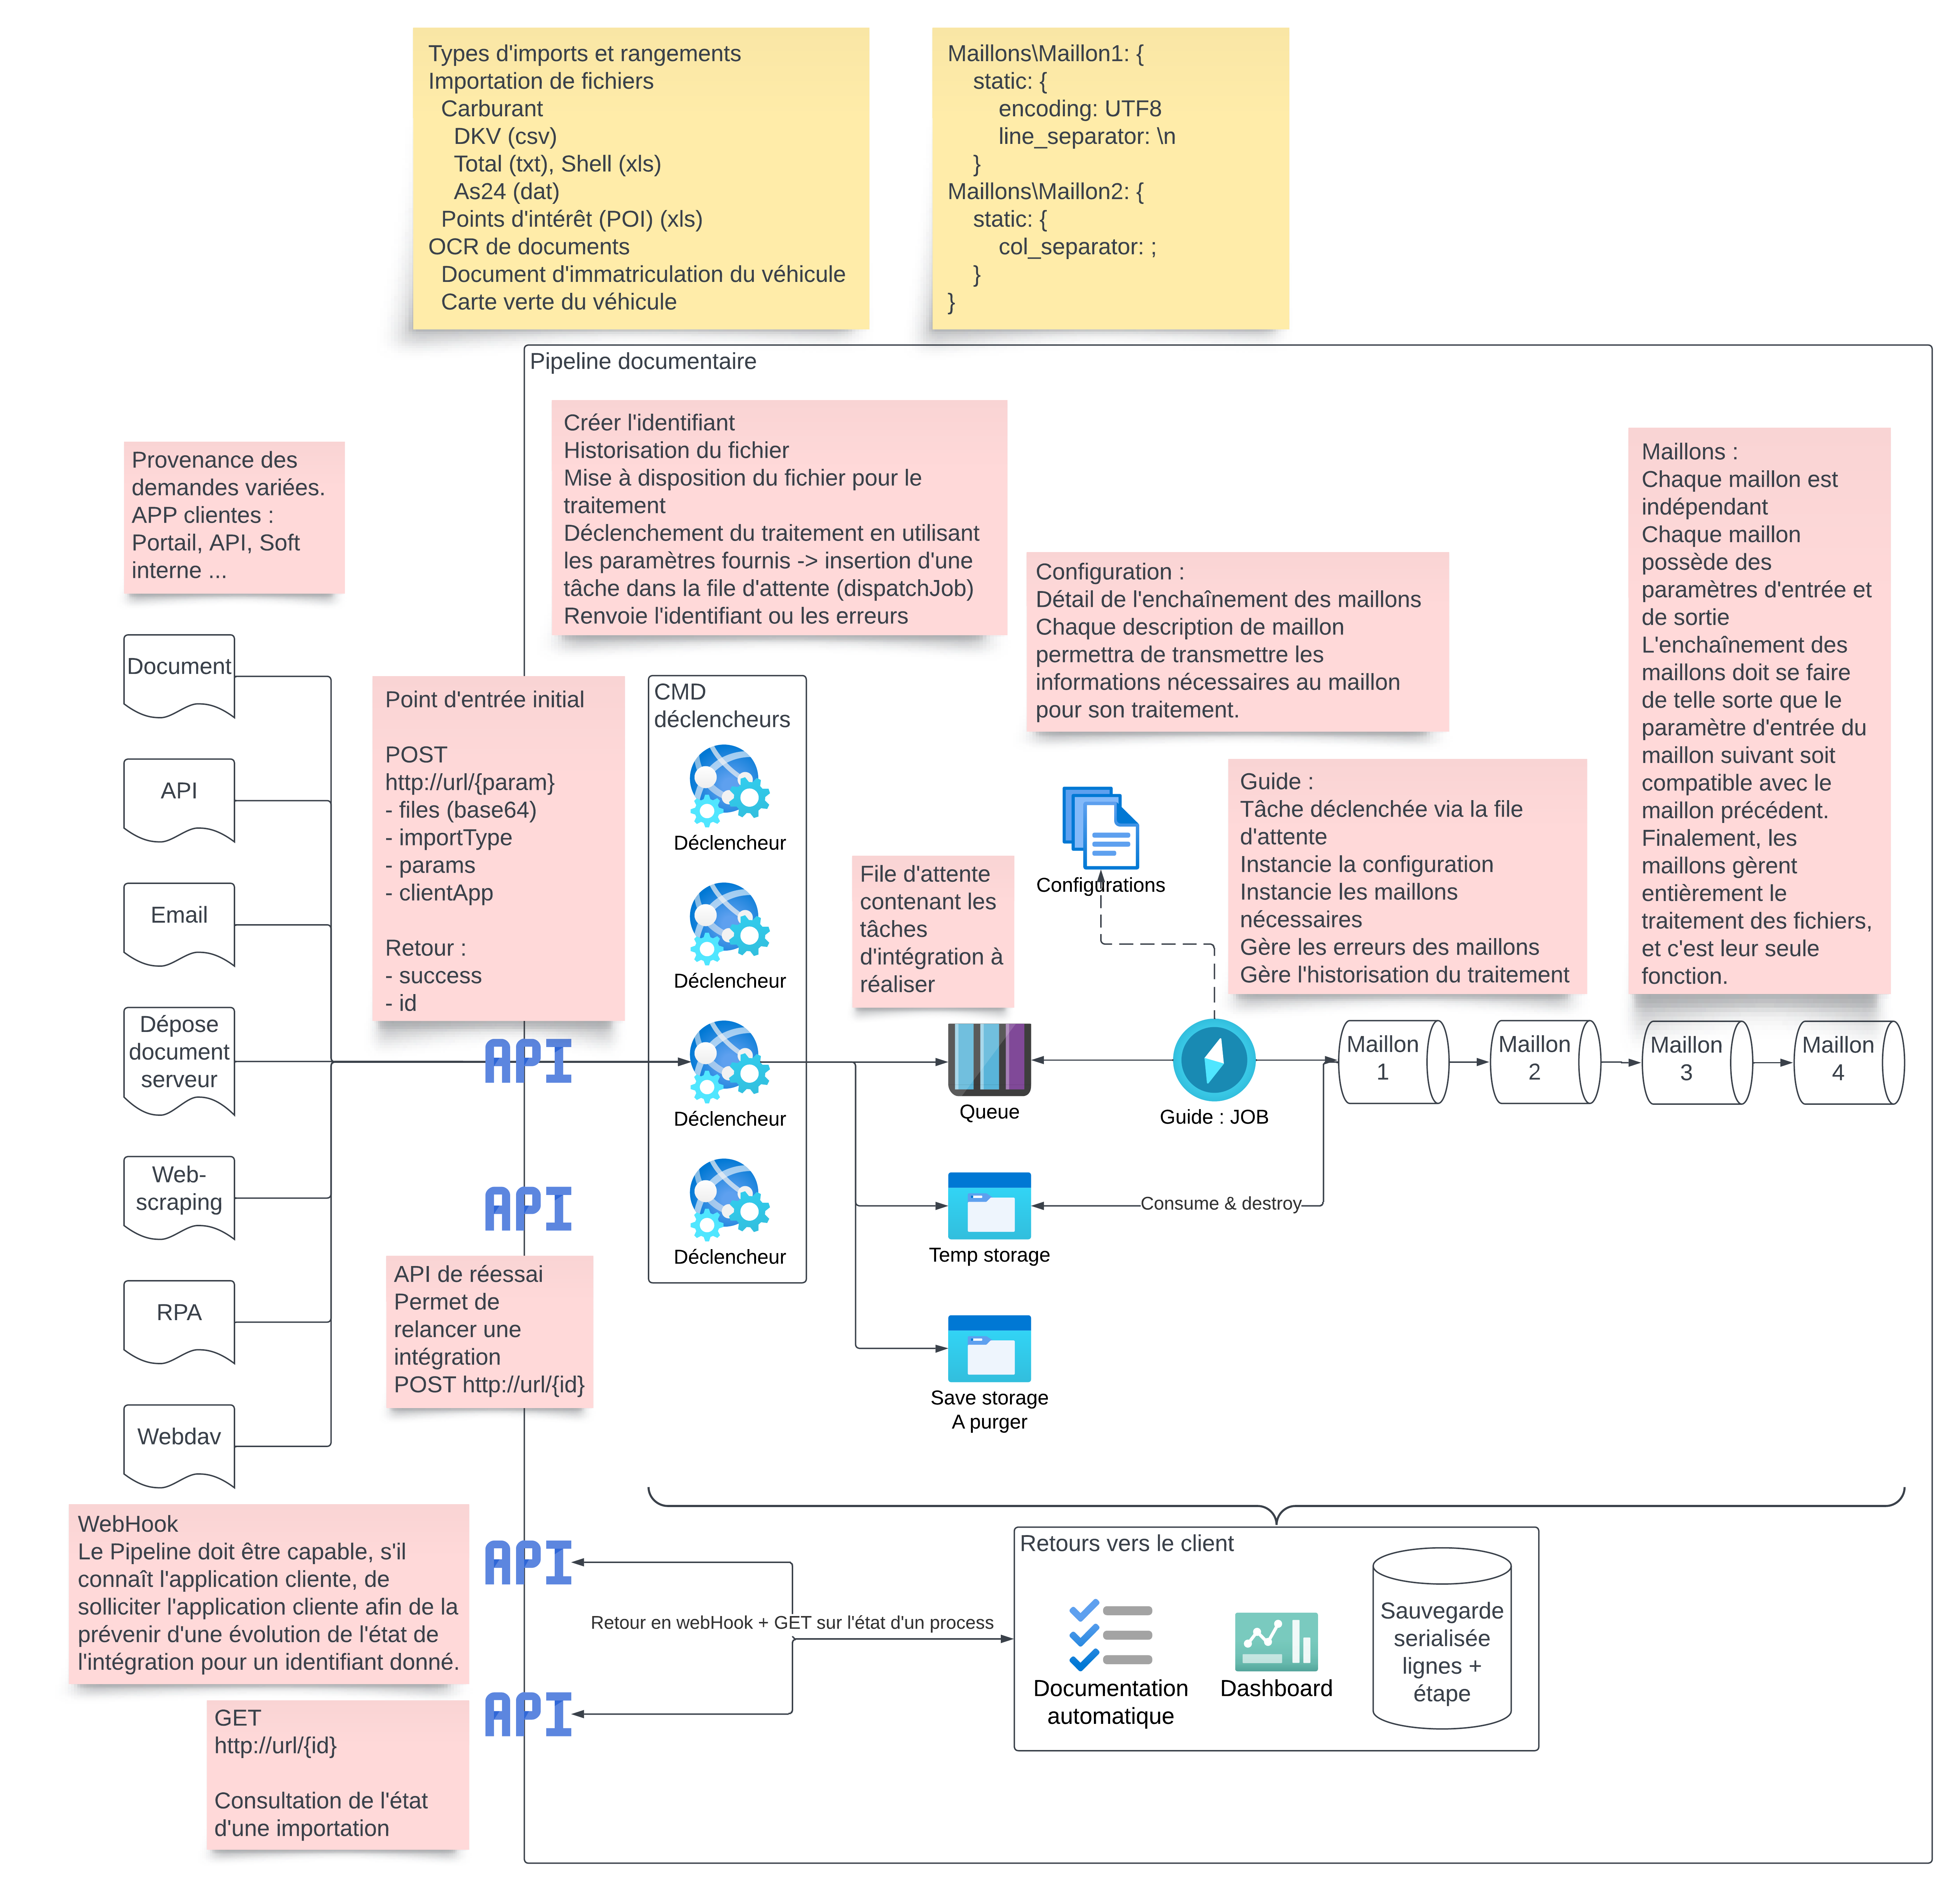
\includegraphics[width=\textwidth]{img/schema-architectural}
    \caption{Schéma architectural de Pipeline documentaire.}
    \label{fig:architectural-schema}
\end{figure}
\chapter{Les spécifications fonctionnelles et techniques}\label{ch:specifications-fonctionnelles-techniques}

J'ai travaillé sur le projet Pipeline documentaire sous la direction de ma tutrice au sein de l'équipe de développement de SuiviDeFlotte. Avant de commencer, étant donné la complexité du projet, nous avons tenu plusieurs réunions avec le propriétaire du produit. Celui-ci nous a expliqué en détail ses idées concernant le projet, et bien sûr, nous avons également partagé nos réflexions.

Dans le chapitre précédent, je crois que c'était évident que notre propriétaire de produit avait une vision précise de la manière dont l'application devait être construite et de son fonctionnement. Par conséquent, nous n'avons pas eu besoin de débuter par l'analyse d'un cahier des charges pour identifier les entités et les relations qu'il pourrait contenir. Cette étape avait déjà été accomplie.

Il a également été convenu que nous développerions ce projet en utilisant le framework Laravel et que nous le déploierions dans des conteneurs Docker. Nous avons constaté que le framework Laravel offrait tous les éléments nécessaires pour ce projet : commandes, gestion des événements, mise en file d'attente des tâches, ainsi que des fonctionnalités pour créer facilement une API, entre autres. De ce fait, ce choix nous est apparu comme judicieux, d'autant plus qu'il avait déjà été utilisé pour de nombreux autres projets au sein de la société, ce qui signifiait que les développeurs possédaient une solide expérience avec cet outil.

L'utilisation de conteneurs Docker pour le développement n'était pas encore une pratique courante au sein de l'entreprise. Cependant, une transition était prévue pour que tous les projets soient conteneurisés. Par conséquent, lors du lancement de nouveaux projets, leur conteneurisation était envisagée dès le début.

Au cours de ces réunions, de plus en plus de détails ont été précisés et nous étions prêts à entamer le projet. Néanmoins, il restait encore un travail de conception à accomplir pour définir en détail l'implémentation de ce projet dans ces cadres.


\chapter{Technologies}\label{ch:technologies}

Au cours du projet Pipeline Documentaire, nous avons choisi diverses technologies pour répondre aux besoins de notre initiative (Figure~\ref{fig:technologies}). En suivant les principes agiles de la méthodologie Scrum, nous avons utilisé Jira pour documenter nos avancées et faciliter la collaboration. Nous avons rassemblé les informations essentielles liées au projet dans Con\-flu\-ence, ce qui a favorisé une meilleure compréhension et une communication fluide au sein de l'équipe.

Pour la gestion des versions, nous avons opté pour git et GitLab, permettant ainsi un suivi précis des modifications et une collaboration simplifiée entre les membres de l'équipe. Dans le domaine du développement, nous avons travaillé avec PHP\-Storm, qui nous a fourni un ensemble d'outils adaptés à nos besoins pour la création d'applications PHP.

Afin de faciliter le déploiement, nous avons utilisé Docker et Docker Compose pour la conteneurisation du projet, ce qui a simplifié la configuration et la maintenance de l'environnement. Le cœur de notre application a été construit avec PHP 8.1 et Laravel 9, offrant une base solide pour nos développements. Nous avons utilisé MariaDB 10 comme base de données en raison de sa stabilité et de ses performances. Pour le serveur web, nous avons choisi Nginx, qui a assuré la distribution efficace de notre application et des temps de réponse rapides. Pour tester notre API, nous avons fait appel à Postman, ce qui nous a permis d'effectuer des tests approfondis pour garantir le bon fonctionnement de chaque composant.

Dans le cadre du projet Gestion de parc (Figure~\ref{fig:architecture}), j'ai travaillé sur la page d'importation des transactions de carburant. Mon objectif était de mettre à jour l'API utilisée pour cette page en utilisant la nouvelle API de Pipeline Documentaire. Pour cela, J'ai réalisé le maquettage avec Figma et j'ai travaillé avec Vue.js et Blade dans le cadre de la mission frontend, en cherchant à offrir une expérience utilisateur améliorée et conviviale.

\begin{figure}[ht]
    \centering
    
\includegraphics[width=0.9\textwidth]{img/technologies01}
    \caption{Les principales technologies utilisées dans le cadre du projet.}
    \label{fig:technologies}
\end{figure}
\chapter{Réalisations}\label{ch:realisations}

Après avoir exploré en détail la conception et la structure de l'API Pipeline documentaire, je me tourne maintenant vers sa réalisation concrète. Ce chapitre mettra en lumière la mise en œuvre pratique du projet, en alignant chaque étape avec les concepts élaborés précédemment. Des exemples de code viendront illustrer la manière dont les idées abstraites se traduisent en fonctionnalités fonctionnelles.

La réalisation de ce chapitre se décompose en deux sections principales. La première section se concentrera sur la démonstration des fonctionnalités clés du Pipeline documentaire. Plutôt que d'expliquer chaque aspect du projet en détail, ce segment mettra en avant les fonctionnalités principales de l'API. En utilisant des extraits de code pertinents, je suivrai l'évolution des composants essentiels, en mettant en évidence leur rôle dans l'importation et le traitement de fichiers.

La seconde section se focalisera sur une mission frontend spécifique qui illustre l'intégration pratique de l'API nouvellement créée. Plus précisément, j'explorerai comment la page d'importation des fichiers de transactions de carburant dans le projet Gestion de parc (Figure~\ref{fig:architecture}, page~\pageref{fig:architecture}) a été modifiée. Plutôt que d'utiliser l'ancienne API, cette page a été adaptée pour tirer parti de la puissance du nouveau Pipeline documentaire. Des exemples de code détaillés montreront comment ces modifications ont été apportées.

En réunissant la théorie et la pratique, ce chapitre offre un aperçu complet de la réalisation du projet, en montrant comment les concepts élaborés ont été traduits en un système fonctionnel.

\section{Pipeline Documentaire}\label{sec:pipeline-documentaire}

Cette première section plonge au cœur du projet Pipeline documentaire. Je commencerai par examiner le processus d'installation du projet dans un environnement de développement. Cela inclura la préparation de l'infrastructure nécessaire (conteneurs Docker) à l'exécution de l'API et la configuration de Laravel. De plus, je me pencherai sur les migrations de base de données indispensables pour assurer la cohérence des données et le bon fonctionnement de l'API. La section se poursuivra en explorant les modèles qui correspondent aux tables de la base de données.

Le cœur de cette section portera sur le processus clé de l'API : l'importation d'un fichier. Je décomposerai ce processus complexe en étapes gérables, en mettant en évidence les opérations importantes qui se produisent en arrière-plan lorsqu'un fichier est soumis à l'API. Des exemples de code accompagneront cette exploration, illustrant chaque étape du processus.

Enfin, j'aborderai l'aspect crucial des tests. La fiabilité et la robustesse de l'API sont essentielles pour assurer un fonctionnement sans faille.

En somme, cette première section plongera profondément dans l'API Pipeline documentaire, de sa mise en place à son fonctionnement concret. Chaque aspect exploré contribuera à la construction d'une base solide pour la section suivante, où j'examinerai l'intégration de l'API dans une mission frontend spécifique.

\subsection{Installation pour le développement}

Pour amorcer le développement de l'API, il est impératif de cloner deux projets à partir du dépôt GitLab de l'entreprise. Le premier de ces projets, intitulé \Verb|pipelinedoc-docker|, renferme un ensemble de fichiers essentiels. Ce dépôt inclut notamment un \Verb|Dockerfile| (\Verb|app.dockerfile|) ainsi qu'un fichier \Verb|docker-compose.yml|. Il abrite également une structure de dossiers (Figure~\ref{fig:pipelinedoc-docker-folders}) comprenant le fichier de configuration Nginx (\Verb|app.conf|), le répertoire destiné au code de l'API (\Verb|apps|) ainsi que d'autres dossiers de substitution nécessaires au projet.

\begin{wrapfigure}{l}{0.32\textwidth}
    \centering
    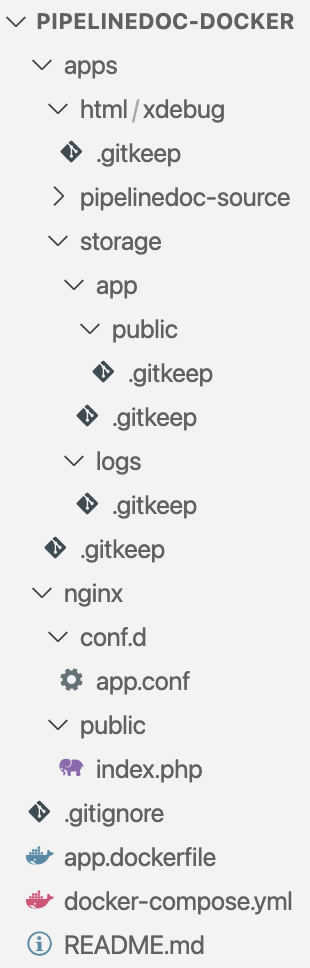
\includegraphics[width=0.30\textwidth]{img/pipelinedoc-docker-folders}
    \caption{La structure des dossiers du projet \Verb{pipelinedoc-docker}.}
    \label{fig:pipelinedoc-docker-folders}
\end{wrapfigure}

Le second projet, baptisé \Verb|pipelinedoc-source|, renferme le code source de l'API Pipeline documentaire. Ce dernier devra être cloné dans le dossier approprié au sein du projet \Verb|pipelinedoc-docker|. Cette étape est primordiale pour établir la connexion entre l'infrastructure Docker mise en place et le code de l'API à développer.

Les fichiers \Verb|app.dockerfile|, \Verb|docker-compose.yml| et le fichier de configuration Nginx sont essentiellement les mêmes que les fichiers présentés pour la production (Code source~\ref{code:dockerfile-prod}, page~\pageref{code:dockerfile-prod}; Code source~\ref{code:docker-compose-prod}, page~\pageref{code:docker-compose-prod}; Code source~\ref{code:nginx-conf-prod}, page~\pageref{code:nginx-conf-prod}). Cependant, bien qu'ils soient plus simples, ils ne contiennent pas toutes les instructions présentes dans ces fichiers.

Dès que les deux projets sont clonés, les conteneurs Docker peuvent être démarrés avec la commande suivante : \Verb|docker compose up|. Ensuite, le développeur doit créer le fichier \Verb|.env| pour le projet, contenant toutes les variables environnementales nécessaires, telles que les détails des connexions à la base de données, les URL et les jetons vers d'autres services, ainsi que d'autres paramètres de configuration. L'étape suivante consiste à installer les dépendances avec la commande \Verb|composer install| et à les mettre à jour avec la commande \Verb|composer update|. Ces commandes utilisent le fichier \Verb|composer.json| pour installer et mettre à jour les dépendances répertoriées avec leurs numéros de version. Ce projet inclut non seulement des dépendances publiques, mais également des dépendances développées et maintenues par l'entreprise dans son propre dépôt privé. Ces paquets privés sont ce que l'on appelle les \foreignquote{french}{cores}, comme nous l'avons mentionné précédemment (Figure~\ref{fig:architecture}, page~\pageref{fig:architecture}; Sous-section~\ref{subsec:cores}, page~\pageref{subsec:cores}).

Il reste encore trois petites étapes pour installer et démarrer complètement le projet : il faut lancer la commande \Verb|php artisan migrate:install|\footnote{Artisan est l'outil de ligne de commande intégré de Laravel, permettant d'effectuer diverses tâches liées au développement et à la gestion de projets Laravel.} pour créer la table \Verb|migrations| dans la base de données. Ensuite, il faut exécuter la commande \Verb|php artisan migrate| pour créer les tables nécessaires au projet, qui sont définies dans les fichiers de migration situés dans le dossier \Verb|database/migrations| du projet Laravel. Enfin, il faut utiliser la commande \Verb|php artisan queue:listen|\footnote{Ces commandes doivent bien sûr être exécutées dans le conteneur de l'application et à partir de son dossier racine.} pour démarrer la file d'attente de Laravel. À ce stade, le système est prêt à importer des fichiers et à exécuter ses autres fonctionnalités. Dans les lignes qui suivent, j'examinerai un peu plus en détail les fichiers de migration qui définissent la structure des tables de la base de données nécessaires au projet.
\subsection{Migrations de la base de données}

Les migrations dans Laravel sont un mécanisme permettant de gérer et de maintenir la structure de la base de données d'une application de manière efficace et contrôlée. Les migrations définissent les schémas des tables de la base de données, ainsi que les modifications ultérieures à ces schémas. Elles offrent un moyen de collaborer entre développeurs en suivant un processus de versionnement pour les modifications de la base de données.

Pour créer une migration, on utilise l'outil de ligne de commande Artisan fourni par Laravel, en exécutant la commande \Verb|php artisan make:migration|. Cette commande génère un fichier de migration dans le répertoire \Verb|database/migrations| du projet. Dans ce fichier, on peut définir les colonnes de la table, les clés étrangères, les index, etc.

Une fois la migration créée, on peut exécuter la commande \Verb|php artisan migrate| pour appliquer les migrations en attente et mettre à jour la base de données selon les schémas définis. Les migrations permettent également de revenir en arrière en cas de besoin avec la commande \Verb|php artisan migrate:rollback|.

L'utilisation des migrations permet aux développeurs de travailler de manière collaborative et organisée en maintenant un historique des changements de structure de la base de données. Cela facilite également le déploiement sur différents environnements et assure une gestion centralisée de la structure de la base de données au sein du code source du projet.

Comme le modèle physique de données (Figure~\ref{fig:pmd}, page~\pageref{fig:pmd}) l'a défini, nous avons créé trois tables dans la base de données à l'aide de fichiers de migration : la table des téléchargements (\Verb|uploads|), la table des étapes des téléchargements (\Verb|upload_step|) et la table des résultats des téléchargements \Verb|upload_results|. À titre d'exemple, le fichier de migration de la table \Verb|uploads| est présenté dans le Code source~\ref{code:uploads-migration}.

Cette migration crée une table nommée \Verb|uploads| avec plusieurs colonnes :

\begin{itemize}
    \item \textbf{\Verb|id|} : Une clé primaire unique générée à l'aide d'ULID (Universally Unique Lexicographically Sortable Identifier).
    \item \textbf{\Verb|parameters|} : Une colonne de type JSON pour stocker des paramètres au format JSON.
    \item \textbf{\Verb|client_app|} : Une colonne de type entier pour enregistrer l'application cliente.
    \item \textbf{\Verb|upload_type|} : Une colonne de type chaîne de caractères (string) pour spécifier le type de téléchargement.
    \item \textbf{\Verb|status|} : Une colonne de type entier avec une valeur par défaut de 0, représentant l'état du téléchargement (0 : reçu, 1 : démarré, 2 : en attente, 3 : terminé, 4 : abandonné).
    \item \textbf{\Verb|timestamps|} : Deux colonnes pour enregistrer les horodatages de création et de mise à jour des enregistrements.
    \item \textbf{\Verb|deleted_at|} : Une colonne pour prendre en charge la suppression douce (soft delete) avec une précision temporelle de 0.
\end{itemize}

\begin{code}
    \caption{La classe de migration de la table \Verb{uploads}.}
    \inputminted{php}{code/2022_12_20_111202_create_uploads_table.php}
    \label{code:uploads-migration}
\end{code}

La méthode \mintinline{php}|up()| est utilisée pour créer la table avec les colonnes spécifiées, tandis que la méthode \mintinline{php}|down()| est utilisée pour supprimer la table en cas de rollback. Le code est encapsulé dans une classe anonyme héritant de la classe de migration. Cela permet de créer et exécuter la migration sans avoir à nommer explicitement la classe de migration, ce qui est courant dans les fichiers de migration Laravel.

L'objet \mintinline{php}|$table|, au sein de la classe de migration, représente l'entité qui permet de définir et de structurer la table de base de données au moyen de la migration. Dans le contexte de Laravel, cet objet est une instance de la classe \mintinline{php}|Blueprint|, qui offre un ensemble de méthodes et de fonctionnalités pour concevoir la structure de la table de manière programmatique.

    Chaque méthode appelée sur l'objet \mintinline{php}|$table| correspond à une opération spécifique permettant de construire la table. Ceci facilite la création cohérente et reproductible de la base de données. Par exemple, dans ce cas, les instructions telles que \mintinline{php}|$table->ulid('id')->primary()| définissent la colonne \Verb|id| comme une clé primaire dotée d'une valeur unique générée par le biais d'ULID. De la même manière, d'autres méthodes comme \mintinline{php}|$table->json('parameters')|, \mintinline{php}|$table->integer('client_app')|, etc., définissent les colonnes de la table et leurs types de données respectifs.

    L'objet \mintinline{php}|$table| revêt une importance fondamentale au sein du processus de migration Laravel. Il agit comme un canal permettant de décrire, de manière systématique, la structure de la table de base de données. Ce mécanisme offre une approche structurée et organisée pour gérer les changements de schéma de la base de données de manière réversible et documentée.

La structure des fichiers de migration des deux autres tables est similaire à celle-ci, avec des colonnes différentes bien sûr. Ces deux tables sont dans une relation un-à-plusieurs avec la table \Verb|uploads|, donc elles ont des clés étrangères comme l'une de leurs colonnes créées par le code suivant dans leurs fichiers de migration : \mintinline{php}|$table->foreignUlid('upload_id')->constrained('uploads');|.

Laravel utilise les informations dans des fichiers des migrations pour générer automatiquement les requêtes SQL nécessaires. Cela se traduit par la création, la modification ou la suppression des tables et des colonnes dans la base de données sous-jacente. Par exemple, le code SQL généré par Laravel à partir du fichier de migration de la table \Verb{uploads} est présenté dans le Code source~\ref{code:uploads-sql}.

\begin{code}
    \caption{Le code SQL généré par Laravel sur la base du fichier de migration de la table \Verb{uploads}.}
    \inputminted{sql}{code/uploads.sql}
    \label{code:uploads-sql}
\end{code}

\begin{enumerate}
    \item POST
          \begin{enumerate}
              \item Step, 1-2 exemples
          \end{enumerate}
    \item Testing
\end{enumerate}

\section{Mission frontend}

\begin{enumerate}
    \item Maquettage
    \item Modal
    \item Importations
\end{enumerate}
\chapter{Présentation d'un jeu d'essai}\label{ch:jeu-essai}

Ce chapitre présente le fonctionnement de l'API Pipeline documentaire illustré par des captures d'écran. Nous suivons le comportement de l'API à travers les étapes suivantes :

\begin{enumerate}
    \item Nous envoyons une requête POST à l'API à l'aide de Postman pour importer un fichier des transactions de carburant, en l'occurrence, un fichier LCCC. Ensuite, Postman affiche la réponse réussie de l'API (code 201, identifiant et statut du téléchargement) (Figure~\ref{fig:postman}).
    \item Dans le terminal du conteneur Docker de l'application, où la file d'attente de Laravel a été préalablement démarrée à l'aide de la commande \Verb|php artisan queue:listen|, nous pouvons voir la liste des maillons au fur et à mesure que la file d'attente les exécute (Figure~\ref{fig:docker}).
    \item Simultanément, dans la base de données de l'application, nous constatons l'ajout d'un nouvel enregistrement dans la table des téléchargements (\Verb|uploads|). De plus, dans la table des maillons de téléchargement (\Verb|upload_steps|), plusieurs nouveaux enregistrements sont créés pour refléter chaque maillon du traitement du fichier (Figure~\ref{fig:uploads_upload_steps}).
    \item Dans la base de données \Verb|suivideflotte|, les données extraites du fichier sont ajoutées à la table \Verb|23-02_gaz_tid_transaction|, et un nouvel enregistrement est créé dans la table \Verb|gaz_tid_import_historique| pour consigner le succès de l'importation du fichier (Figure~\ref{fig:transaction_history}).
    \item Dans le dossier de stockage (\Verb|storage|) du projet \Verb|docker-pipeline|, le fichier d'origine ainsi que la charge utile sont enregistrés dans le répertoire \Verb|app/storage-directory|, tandis que les fichiers de sortie des différents maillons sont stockés dans le répertoire \Verb|app/work-directory| (Figure~\ref{fig:step-files}).
    \item Enfin, si nous retournons à Postman et tentons d'envoyer une charge utile qui ne contient pas toutes les données requises, l'API répondra avec une erreur 422 (Figure~\ref{fig:postman-error}).
\end{enumerate}

On voit que ce fonctionnement correspond aux exigences initiales formulées dans le cahier des charges du projet.

\begin{figure}[ht]
    \centering
    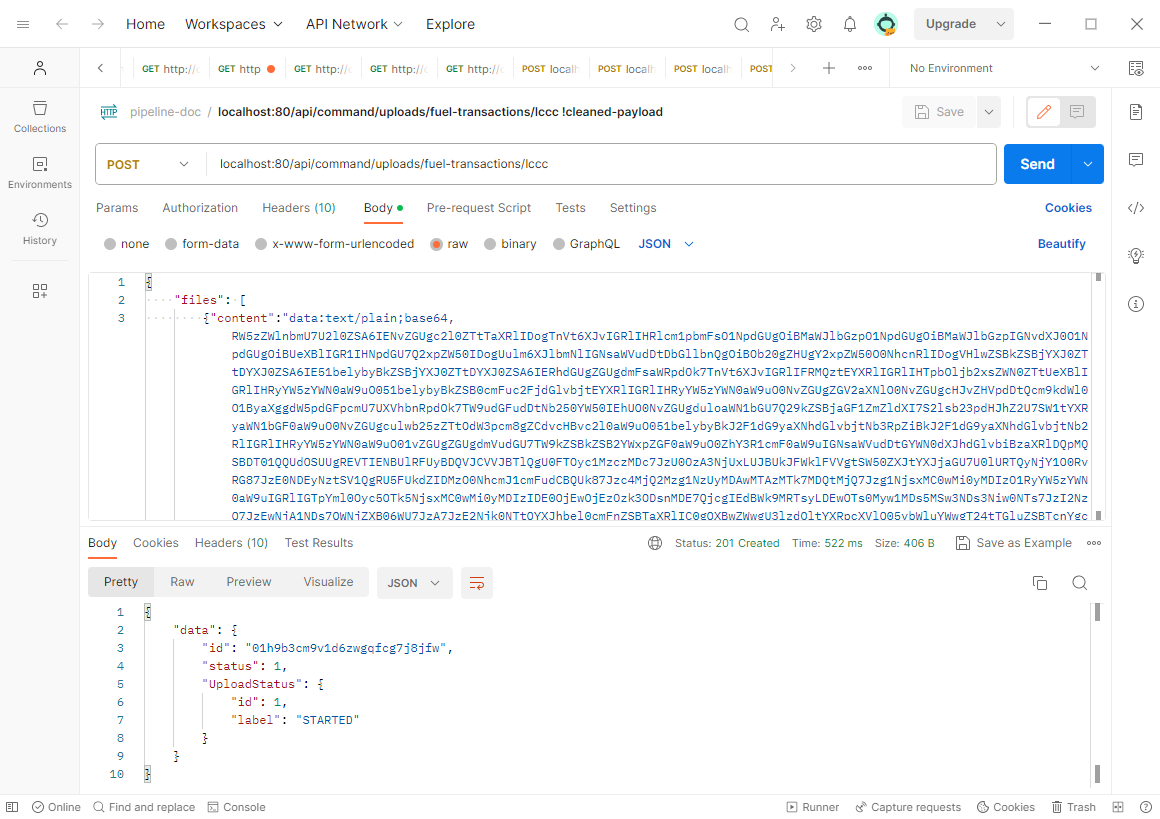
\includegraphics[width=\textwidth]{img/postman}
    \caption{Envoi d'un fichier LCCC à l'API Pipeline documentaire et réception d'une réponse réussie dans Postman.}
    \label{fig:postman}
\end{figure}

\begin{figure}[ht]
    \centering
    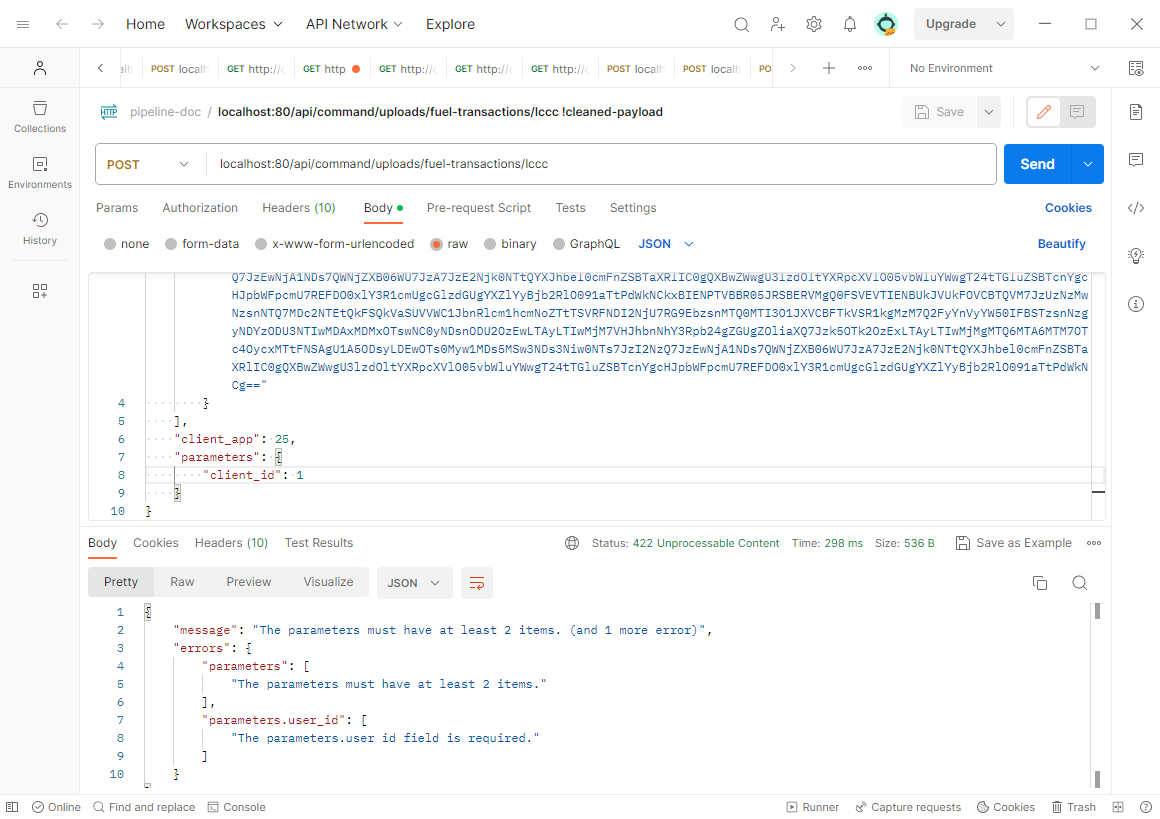
\includegraphics[width=\textwidth]{img/postman-error}
    \caption{L'API répond avec un code d'erreur (422) si nous envoyons un payload non complet (le \Verb{user_id} est manquant).}
    \label{fig:postman-error}
\end{figure}

\begin{figure}[ht]
    \centering
    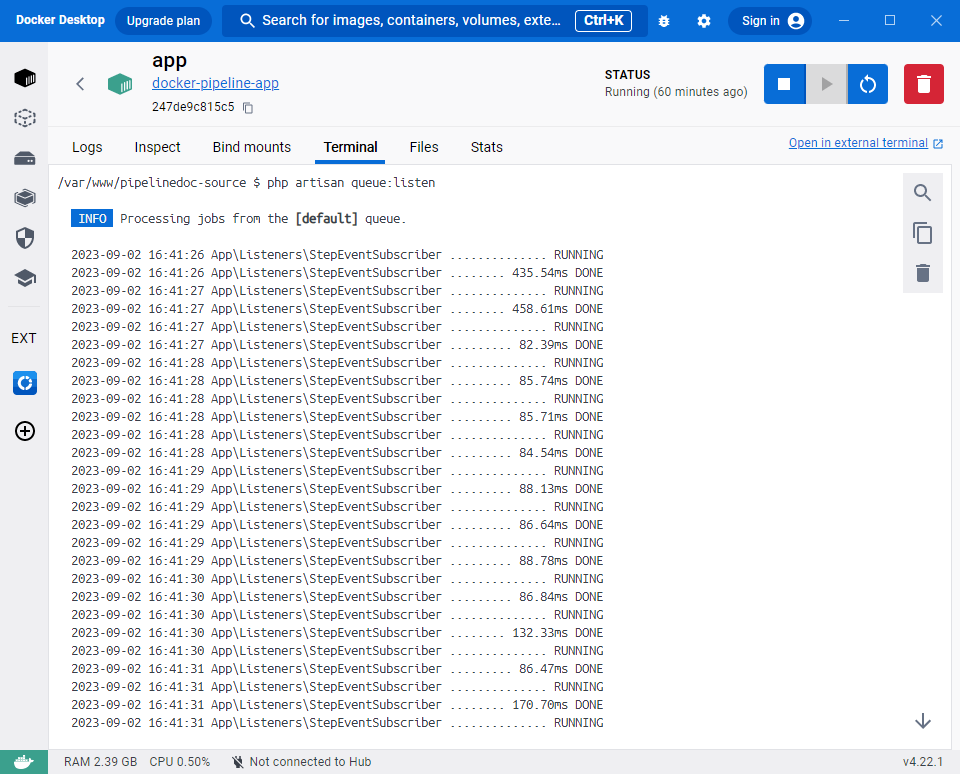
\includegraphics[width=\textwidth]{img/docker}
    \caption{Dans le terminal du conteneur Docker de l'application la liste des maillons est affichée au fur et à mesure que la file d'attente les exécute.}
    \label{fig:docker}
\end{figure}

\begin{figure}[ht]
    \centering
    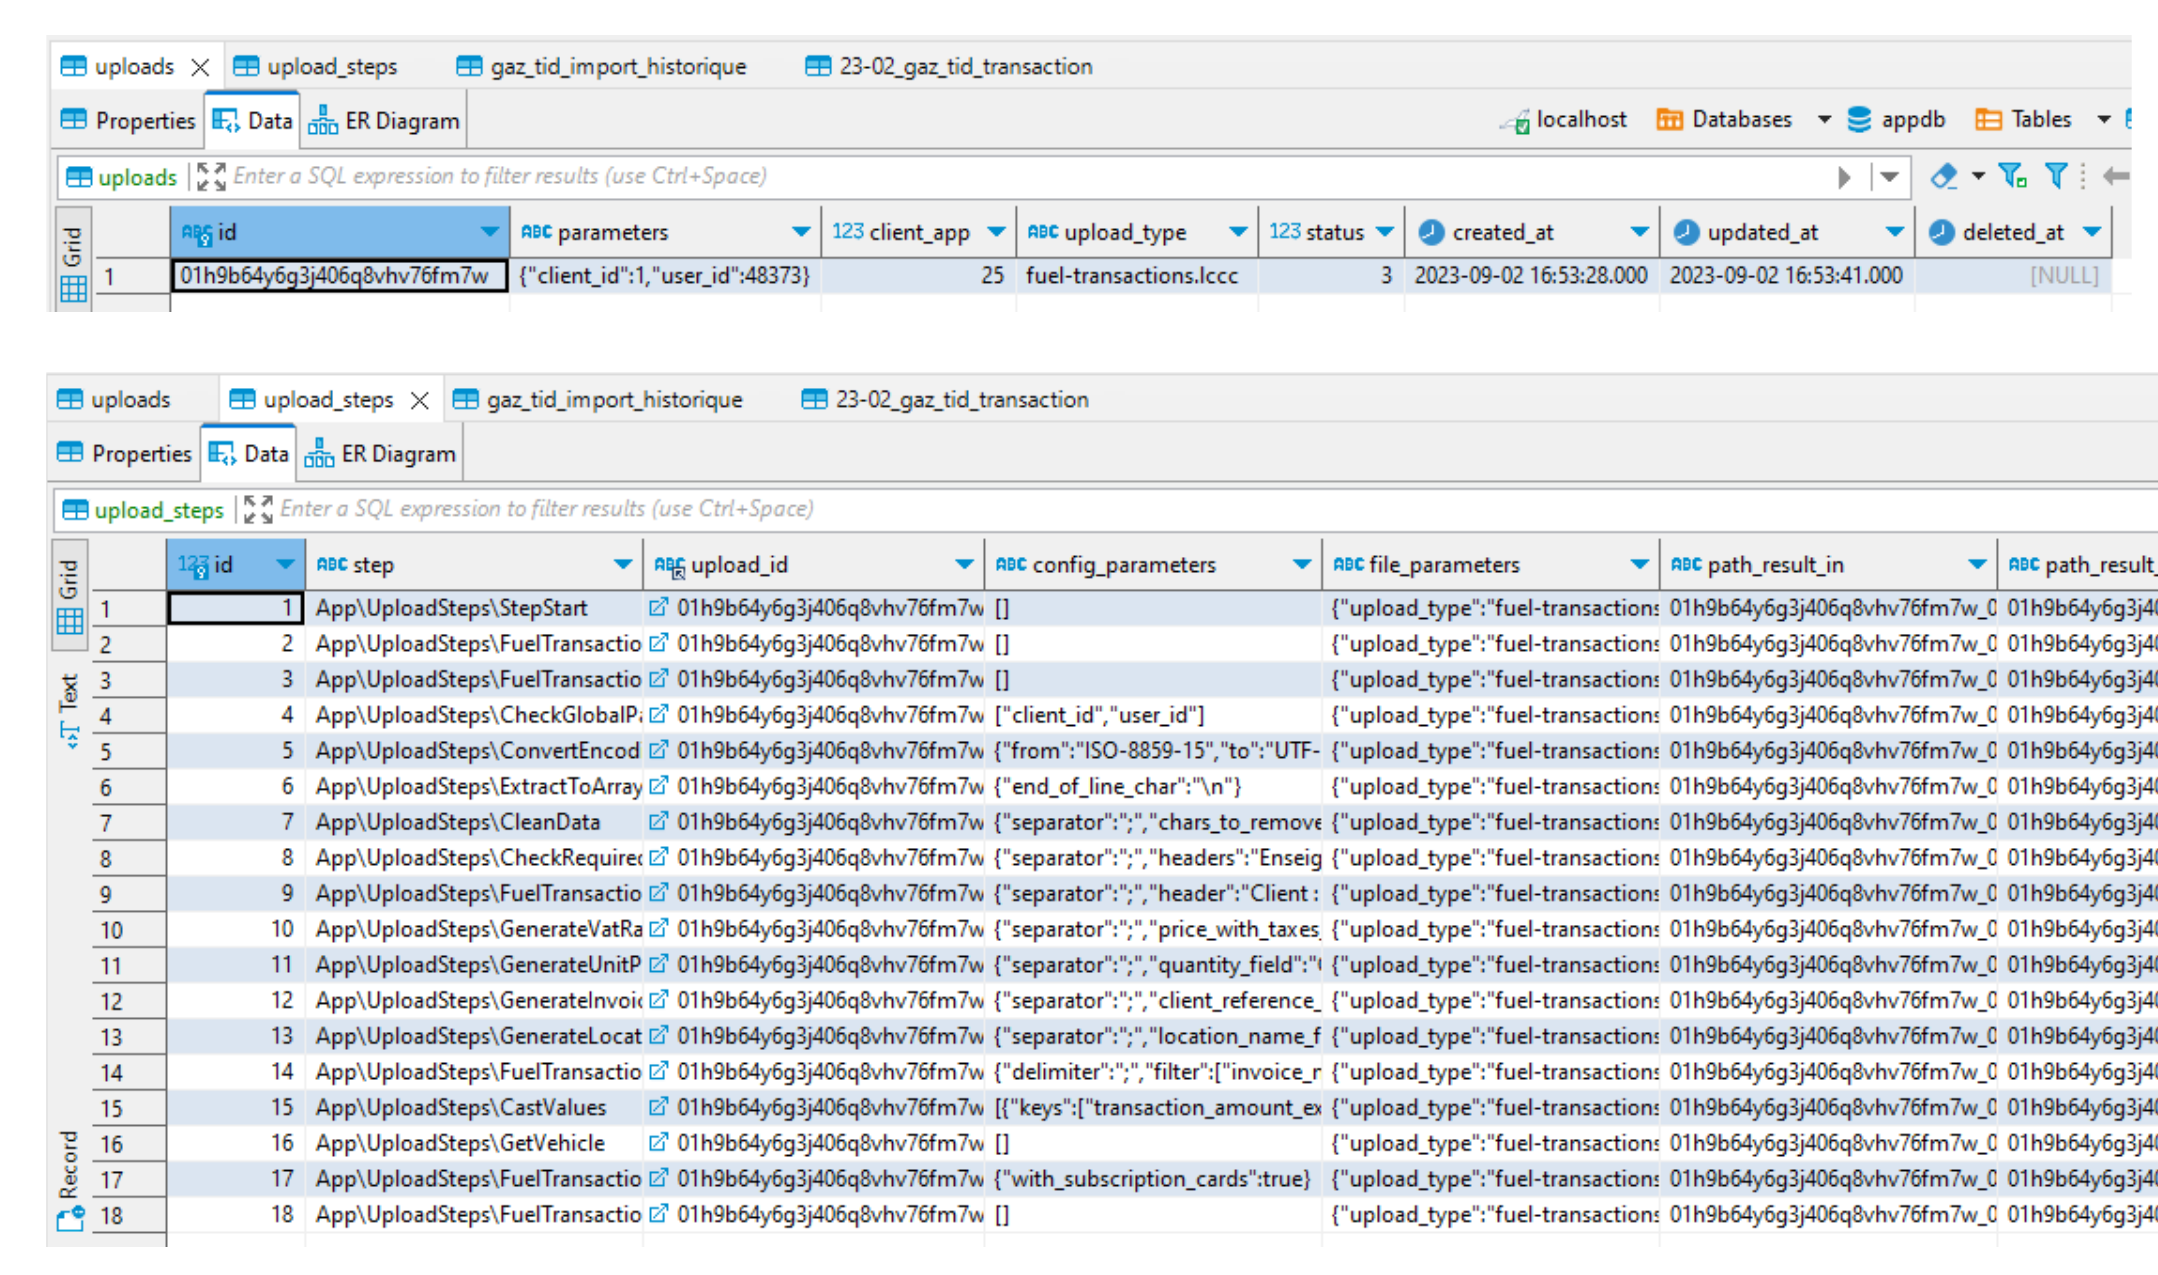
\includegraphics[width=\textwidth]{img/uploads_upload_steps}
    \caption{L'objet \Verb{Upload} et les objets \Verb{UploadStep} sont stockés dans les tables correspondantes de la base de données.}
    \label{fig:uploads_upload_steps}
\end{figure}

\begin{figure}[ht]
    \centering
    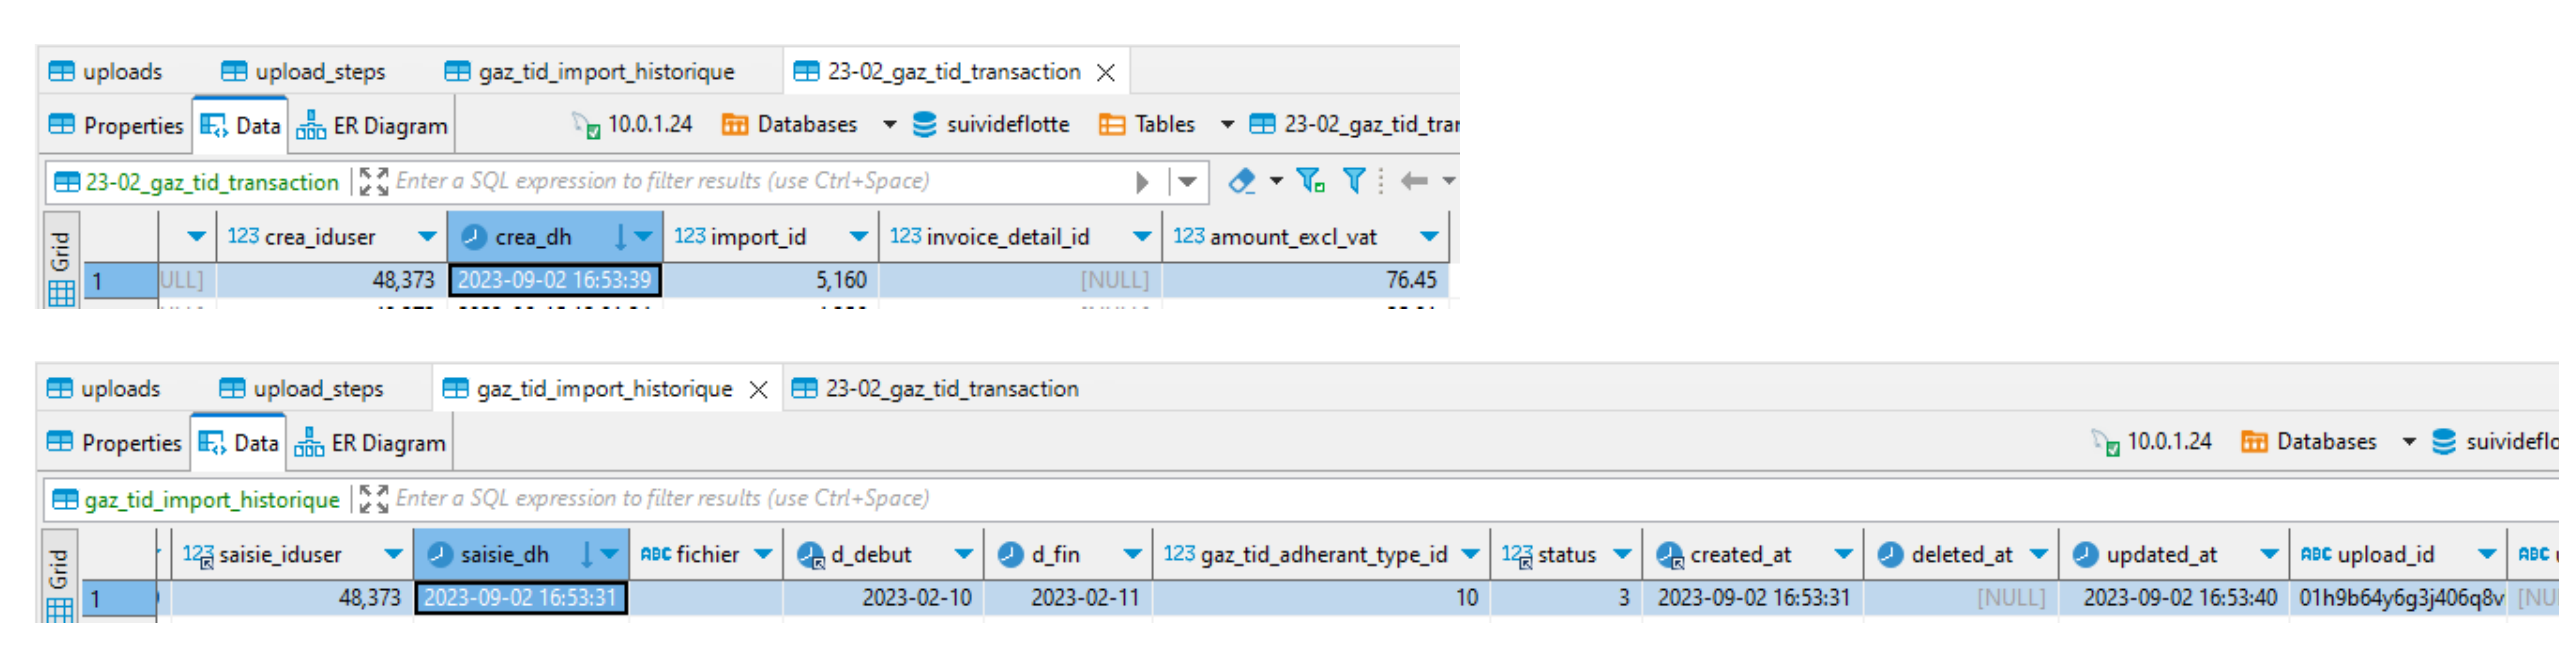
\includegraphics[width=\textwidth]{img/transaction_history}
    \caption{Dans la base de données \Verb{suivideflotte}, les données extraites du fichier sont ajoutées à la table \Verb{23-02_gaz_tid_transaction}, et un nouvel enregistrement est créé dans la table \Verb{gaz_tid_import_historique}.}
    \label{fig:transaction_history}
\end{figure}

\begin{figure}[ht]
    \centering
    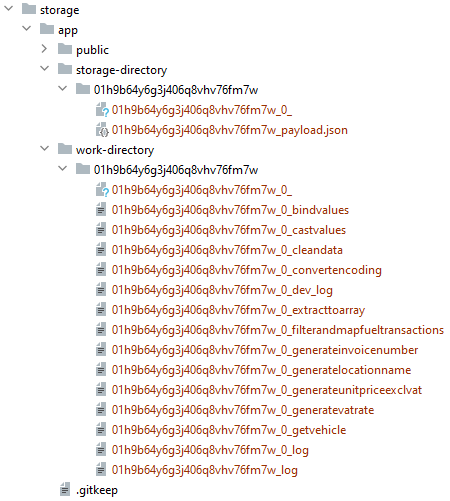
\includegraphics[width=0.9\textwidth]{img/step-files}
    \caption{Dans le dossier de stockage (\Verb{storage}) du projet \Verb{docker-pipeline}, le fichier d'origine ainsi que la charge utile sont enregistrés dans le répertoire \Verb{app/storage-directory}, tandis que les fichiers de sortie des différents maillons sont stockés dans le répertoire \Verb{app/work-directory}.}
    \label{fig:step-files}
\end{figure}
\chapter{Veille sur les vulnérabilités de sécurité}\label{ch:veille-vulnerabilites-securite}
\chapter[Travaux de recherches]{Description d'une situations de travail ayant nécessité des travaux de recherches}\label{ch:recherche}

Au cours de mon alternance, à un moment donné, lorsque le projet Pipeline documentaire était opérationnel et mis en production, le propriétaire du produit m'a confié la tâche de trouver des solutions pour documenter une API créée sous Laravel. Cette documentation serait utile non seulement pour Pipeline documentaire, mais également pour d'autres APIs de l'entreprise qui étaient développées en Laravel.

J'ai commencé mes recherches et j'ai découvert trois packages prometteurs spécialement conçus à cet effet : \Verb{mpociot/laravel-apidoc-generator}, \Verb{rakutentech/laravel-request-docs} et \Verb{darkaonline/l5-swagger}. Après les avoir installés et testés, j'ai créé une documentation complète de Pipeline documentaire en utilisant \Verb{darkaonline/l5-swagger} et \Verb{rakutentech/laravel-request-docs}. Ensuite, j'ai rédigé un rapport dans lequel je les ai comparés en détail.

Vous trouverez ci-dessous les résultats de mes recherches.

\subsubsection{Comparaison}

\paragraph{\Verb{mpociot/laravel-apidoc-generator}}

\begin{itemize}
    \item \Verb{mpociot/laravel-apidoc-generator} est un package populaire pour générer une documentation d'API dans Laravel.
    \item Il utilise des \emph{annotations} dans le code Laravel pour générer automatiquement la documentation.
    \item Le package fournit un ensemble de \emph{commandes Artisan} qui analysent le code source et génèrent une documentation \Verb{HTML} ou \Verb{Markdown}.
    \item Il prend en charge la documentation des \emph{routes}, des \emph{structures de requêtes/réponses}, de \emph{l'authentification}, et bien plus encore.
    \item La documentation générée est \emph{personnalisable} à l'aide de modèles, ce qui nous permet de modifier l'apparence et la structure.
    \item Il prend en charge plusieurs formats de sortie tels que \Verb{HTML}, \Verb{Markdown}, les collections Postman et les spécifications \emph{Swagger/OpenAPI}.
    \item \Verb{mpociot/laravel-apidoc-generator} bénéficie d'une \emph{bonne communauté} de soutien et \emph{il a été régulièrement mis à jour jusqu'au 12/11/2020}.
\end{itemize}

\paragraph{\Verb{darkaonline/l5-swagger}}

\begin{itemize}
    \item \Verb{darkaonline/l5-swagger} est un autre package Laravel \emph{populaire} pour générer une documentation d'API.
    \item Il utilise la spécification \emph{Swagger/OpenAPI} pour documenter les APIs Laravel.
    \item Le package s'intègre aux \emph{routes}, \emph{contrôleurs} et \emph{modèles} Laravel pour générer automatiquement la documentation de l'API.
    \item Il fournit une \emph{interface Swagger UI} où nous pouvons consulter et interagir avec la documentation générée.
    \item \Verb{darkaonline/l5-swagger} prend en charge les \emph{annotations Swagger} pour un contrôle précis du processus de génération de la documentation (Code source~\ref{code:l5swagger}).
    \item Il nous permet de \emph{personnaliser l'apparence de la documentation} en utilisant des thèmes et des options de configuration.
    \item Le package prend en charge l'exportation de la documentation au format \Verb{JSON} ou \Verb{YAML}, qui peut être utilisée avec d'autres outils ou services prenant en charge les spécifications Swagger/OpenAPI.
    \item \Verb{darkaonline/l5-swagger} est \emph{régulièrement mis à jour} et bénéficie d'une \emph{base d'utilisateurs importante}.
\end{itemize}

\paragraph{\Verb{rakutentech/laravel-request-docs}}

\begin{itemize}
    \item \Verb{rakutentech/laravel-request-docs} est un package Laravel spécialement conçu pour \emph{documenter les règles de validation des requêtes}.
    \item Il extrait \emph{automatiquement} les règles de validation des requêtes à partir des contrôleurs Laravel et génère la documentation.
    \item Le package fournit \emph{une commande Artisan} pour analyser le code source et générer une documentation en \Verb{Markdown} ou en \Verb{JSON}.
    \item Il prend en charge la documentation des paramètres de requête (\emph{request parameters}, \emph{query parameters}), des \emph{en-têtes de requêt}e et des \emph{structures de réponse}.
    \item La documentation générée comprend des \emph{exemples de requêtes et de réponses} basés sur les règles de validation.
    \item \Verb{rakutentech/laravel-request-docs} nous permet de \emph{personnaliser} la structure et l'apparence de la documentation à l'aide de modèles.
    \item Il prend en charge l'exportation de la documentation au format \Verb{JSON} pour son intégration avec d'autres outils ou services.
    \item Le package est \emph{régulièrement mis à jour} mais a une \emph{base d'utilisateurs plus réduite} par rapport aux deux autres.
\end{itemize}

En résumé, \Verb{mpociot/laravel-apidoc-generator} et \Verb{darkaonline/l5-swagger} sont des solutions plus complètes pour générer une documentation d'API dans Laravel. Ils s'intègrent aux /emph{routes}, aux /emph{contrôleurs} et aux \emph{modèles}, et prennent en charge \emph{plusieurs formats de sortie}. En revanche, \Verb{rakutentech/laravel-request-docs} est un package spécialisé qui se concentre sur la documentation des \emph{règles de validation des requêtes}.

\begin{code}
    \caption{La fonction \Verb{upload} de la classe \Verb{UploadController} avec des attributs qui peuvent être utilisés par le package \Verb{darkaonline/l5-swagger} pour générer la documentation de l'API.}
    \inputminted[startinline,firstnumber=309]{php}{code/upload-function-L5Swagger.php}
    \label{code:l5swagger}
\end{code}
\chapter{Conclusion}\label{ch:conclusion}

Cette année d'alternance a été une expérience extrêmement enrichissante pour moi. J'ai acquis de nombreuses compétences à l'école, au CEFIM, ainsi qu'au sein de l'entreprise. Elle m'a offert une perspective beaucoup plus large que celle que j'avais avant, même après ma formation de développeur web. J'ai appris énormément sur le développement en général, la programmation orientée objet, la conceptualisation d'un logiciel, la gestion de projet, le DevOps, et bien d'autres domaines, tout cela dans le monde réel.

Mon travail au sein de l'entreprise a été particulièrement formateur, car j'ai eu l'opportunité de travailler sur un projet Laravel depuis ses débuts jusqu'à sa mise en production. En parallèle, j'ai également pu contribuer à des projets existants, ce qui a élargi encore davantage mes compétences.

Tout au long de cette année, j'ai bénéficié d'un excellent soutien de la part de mes enseignants au CEFIM, ainsi que de ma tutrice, de mon propriétaire du produit et de mes collègues au sein de l'entreprise. En regardant en arrière, je ressens une grande satisfaction d'avoir atteint les objectifs fixés au début de cette année d'alternance.

Ce fut un véritable plaisir d'apprendre et de travailler au sein de l'équipe de mes collègues. Je suis impatient de poursuivre mon voyage d'apprentissage continu en rejoignant l'entreprise CHStudio en tant que développeur PHP. Cette nouvelle étape marque le début d'une nouvelle aventure professionnelle, et je suis enthousiaste à l'idée de relever de nouveaux défis et d'approfondir mes compétences dans le domaine du développement web. Je tiens à remercier chaleureusement toutes les personnes qui ont contribué à cette année d'alternance réussie et qui m'ont soutenu tout au long de ce parcours.
\chapter{Remerciements}\label{ch:remerciements}
\begin{appendices}

    \chapter{Gestion de projet}\label{ch-a:gestion-projet}

    \section[Jira : L'outil pour la gestion de projet]{Jira : L'outil essentiel pour la gestion quotidienne de projet}\label{sec-a:jira}

    \begin{figure}[ht]
        \centering
        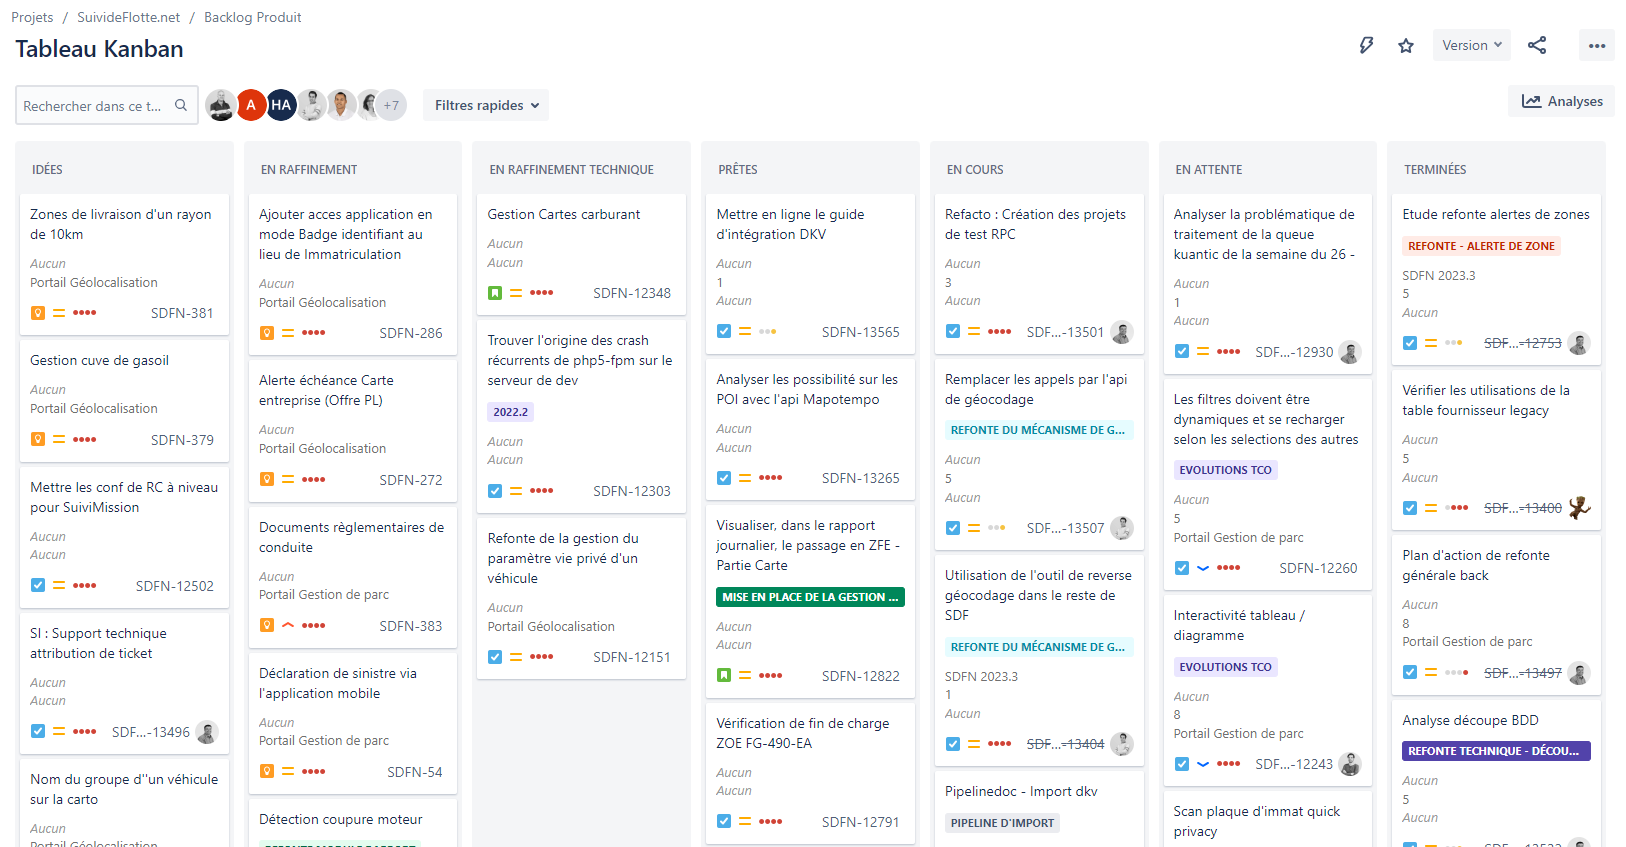
\includegraphics[width=\textwidth]{img/product-backlog}
        \caption{Le Backlog de produit sous forme de tableau Kanban dans Jira.}
        \label{fig:product-backlog}
    \end{figure}

    \begin{figure}[ht]
        \centering
        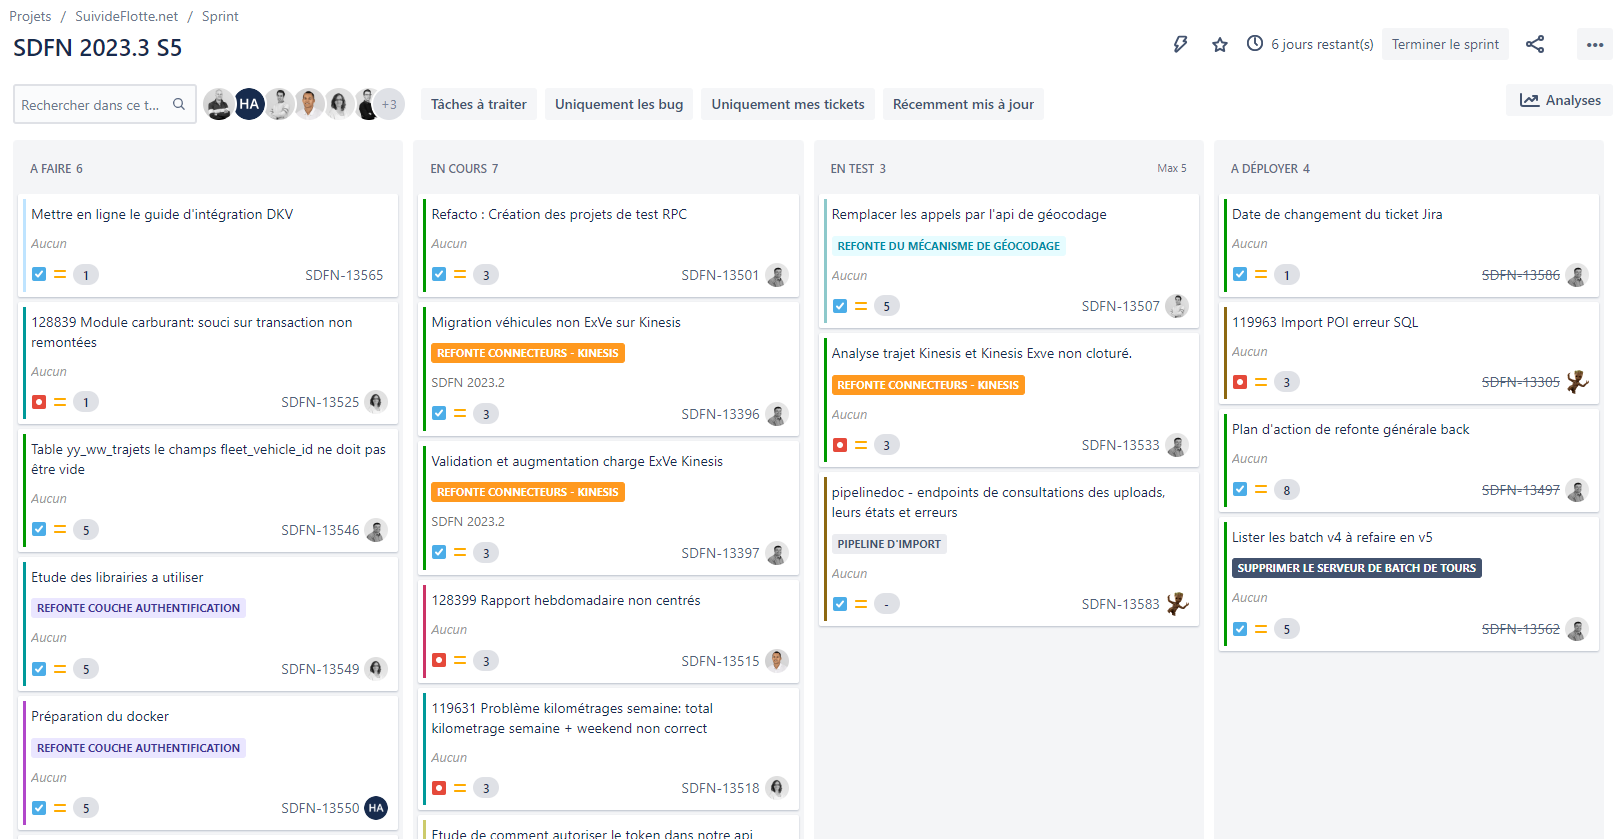
\includegraphics[width=\textwidth]{img/sprint}
        \caption{Le Backlog de sprint sous forme de tableau Kanban dans Jira.}
        \label{fig:sprint-backlog}
    \end{figure}

    \begin{figure}[ht]
        \centering
        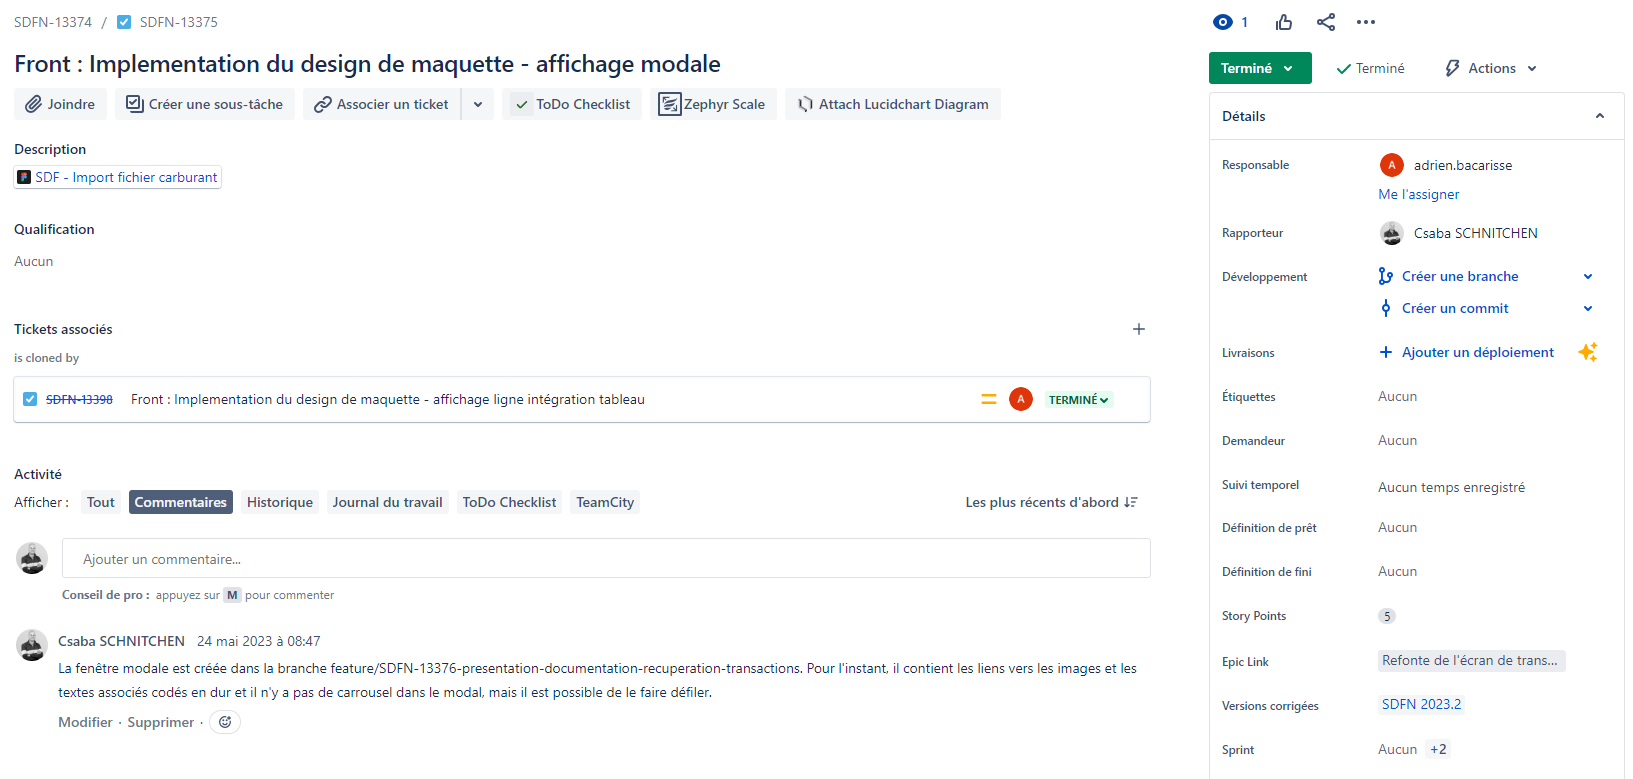
\includegraphics[width=\textwidth]{img/ticket}
        \caption{Un exemple de ticket dans Jira pour le projet d'amélioration de la page d'importation des fichiers des transactions de carburant.}
        \label{fig:ticket}
    \end{figure}

    \begin{figure}[ht]
        \centering
        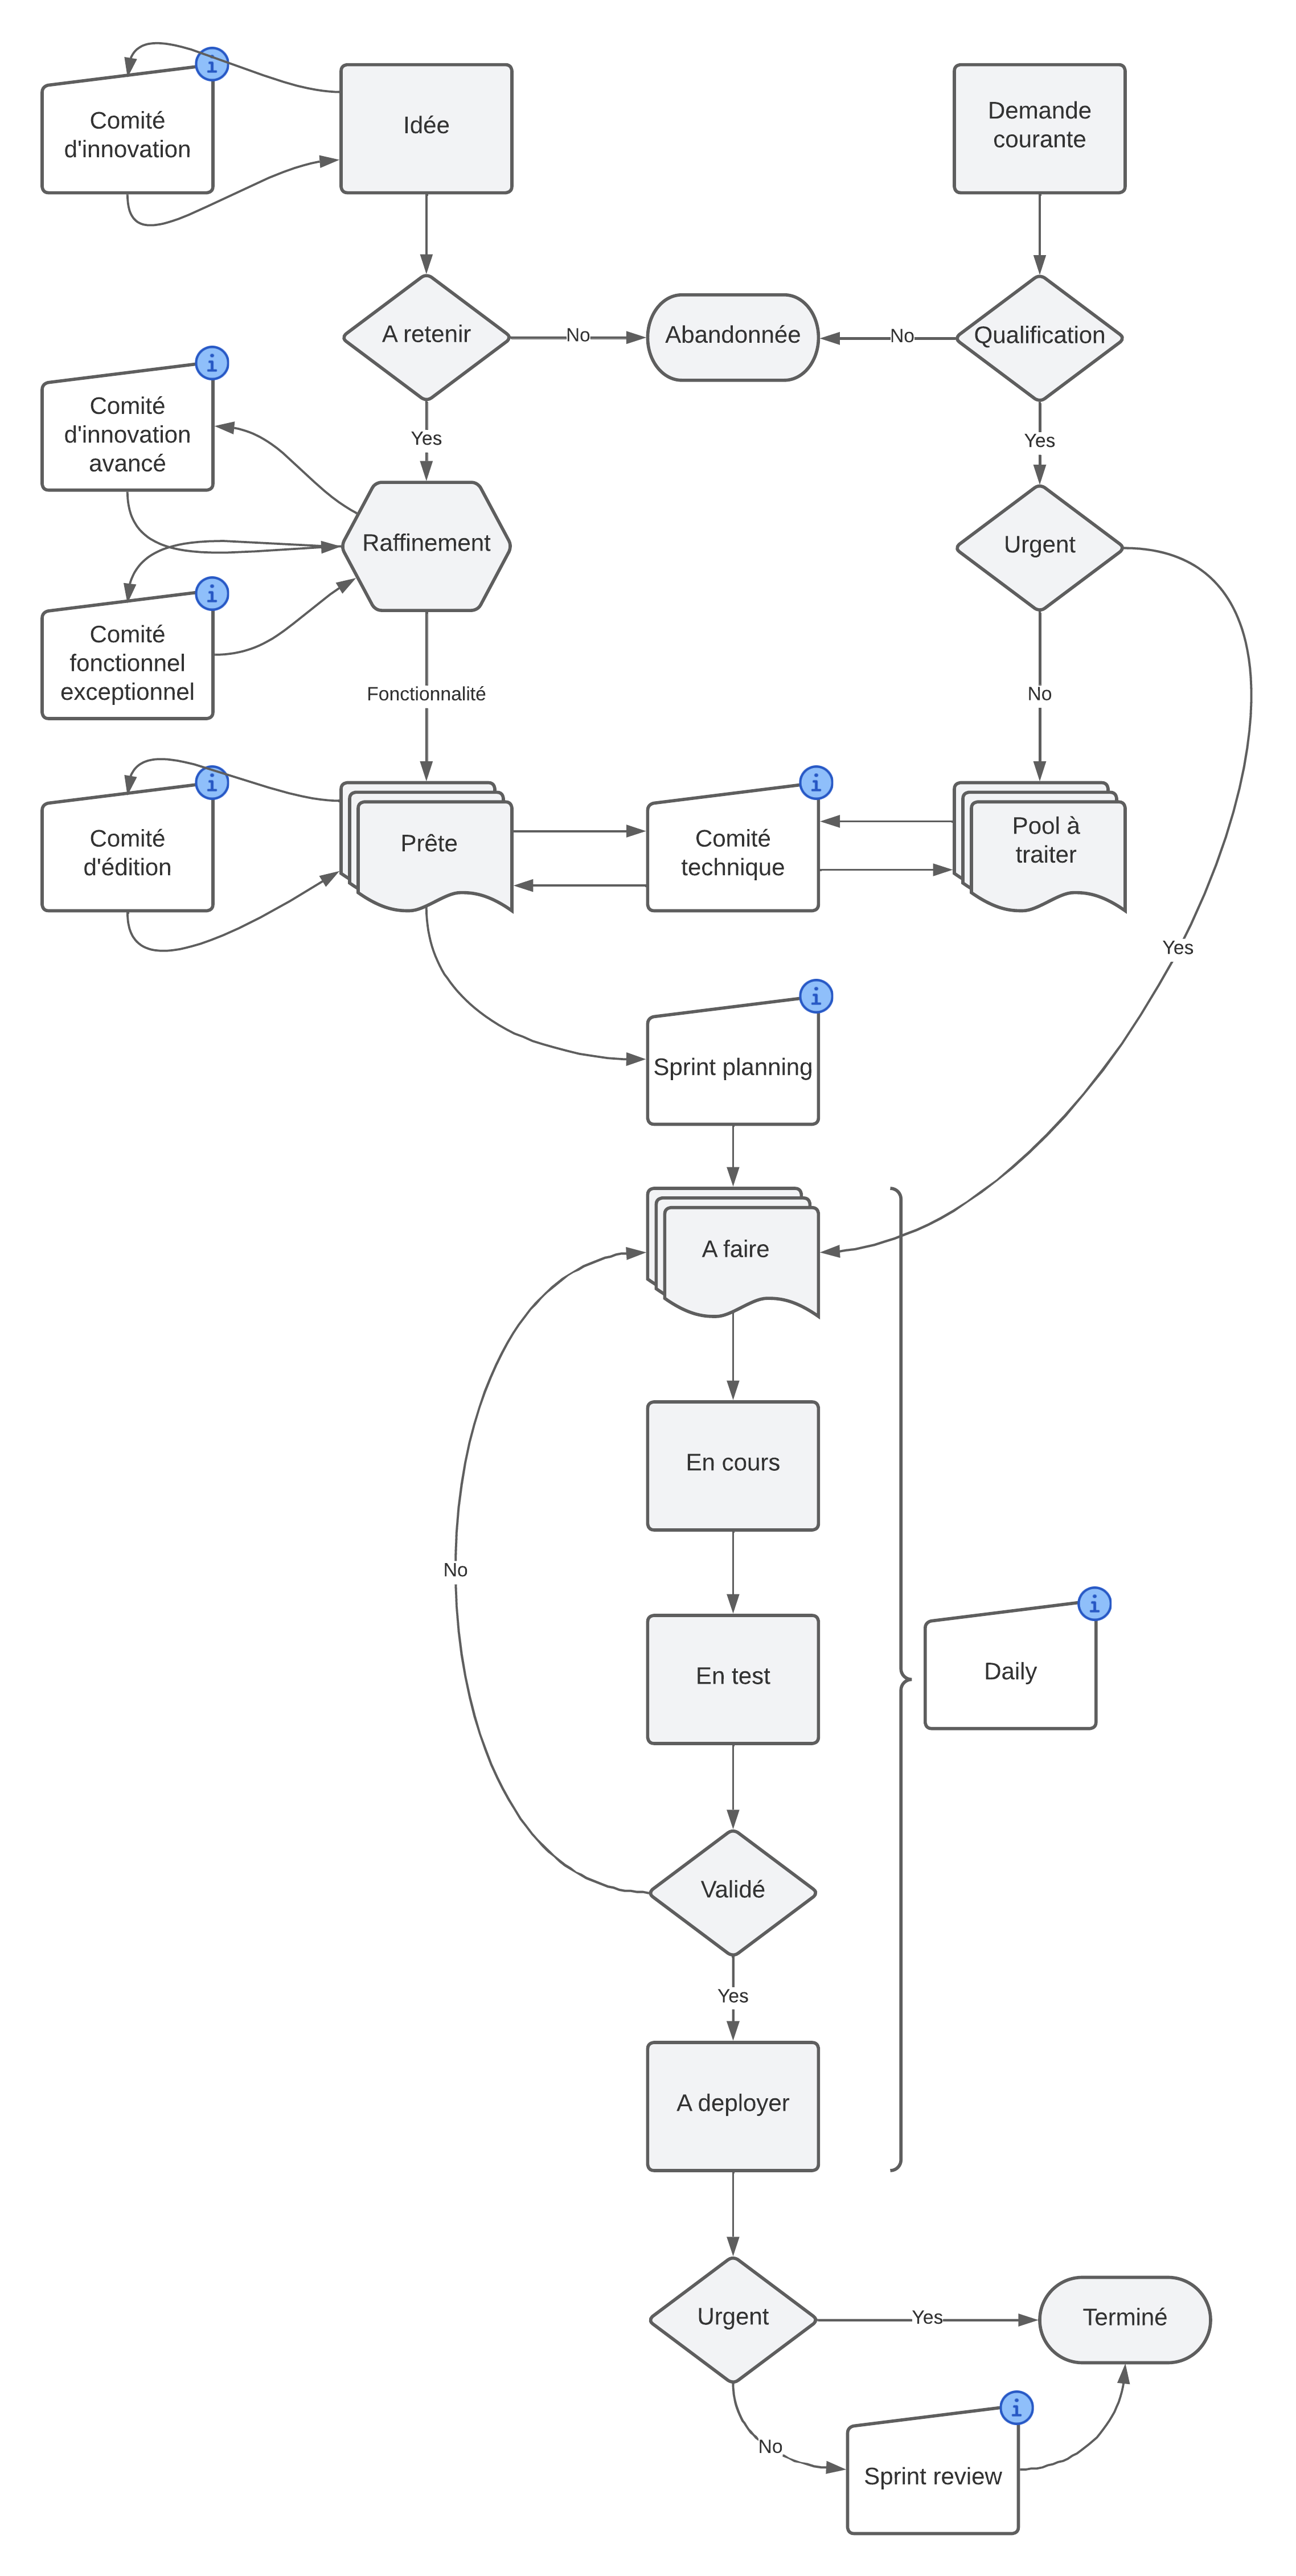
\includegraphics[height=0.94\textheight]{img/lifecycle-of-incoming-ideas}
        \caption{Diagramme d'activité du traitement des idées et des bogues (demandes courantes) entrants chez SuiviDeFlotte.}
        \label{fig:lifecycle-of-incoming-ideas}
    \end{figure}

    \begin{figure}[ht]
        \centering
        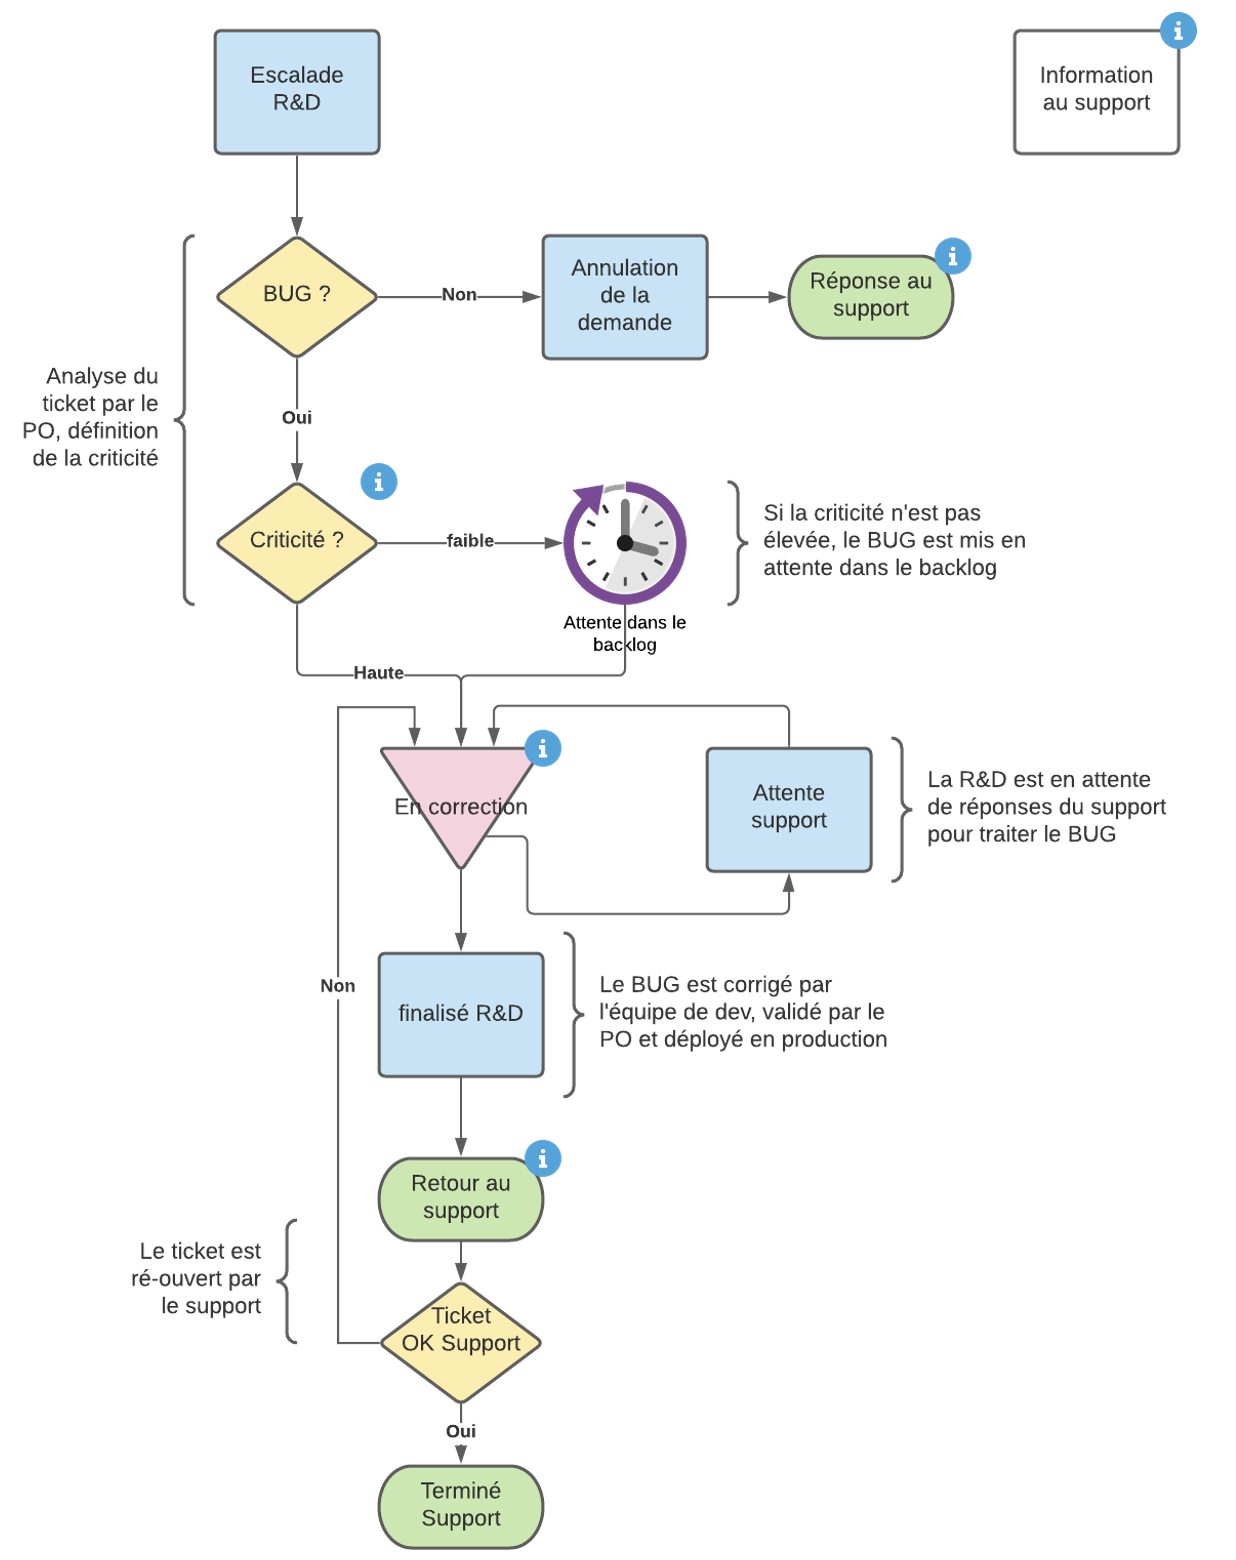
\includegraphics[width=\textwidth]{img/lifecycle-of-bugs}
        \caption{Diagramme d'activité du traitement des bogues.}
        \label{fig:lifecycle-of-bugs}
    \end{figure}

    \section{Intégration Continue et Déploiement Continu}\label{sec-a:ci-cd}

    \begin{code}
        \caption{Le fichier de configuration de Nginx (\Verb{conf.d}) du projet Pipeline documentaire utilisé en production.}
        \inputminted{nginx}{code/conf.d}
        \label{code:nginx-conf-prod}
    \end{code}

    \chapter{Pipeline Documentaire}

    \section{Les événements}

    \begin{code}
        \caption{La classe \Verb{UploadType}.}
        \inputminted{php}{code/UploadType.php}
        \label{code:upload-type}
    \end{code}

    \begin{code}
        \caption{La configuration de l'importation du fichier LCCC.}
        \inputminted{php}{code/lccc.php}
        \label{code:lccc-config}
    \end{code}

    \section{Testing}

    \begin{code}
        \caption{La classe \Verb{CheckEmailTest}.}
        \inputminted{php}{code/CheckEmailTest.php}
        \label{code:check-email-test}
    \end{code}

    \begin{code}
        \caption{Le classe \Verb{UploadControllerTest}.}
        \inputminted{php}{code/UploadControllerTest.php}
        \label{code:upload-controller-test}
    \end{code}

    \chapter{Mission frontend}

    \section{Frontend}

    \begin{code}
        \caption{La partie du fichier \Verb{.diff} téléchargé depuis GitLab qui montre le code du nouveau formulaire d'importation.}
        \inputminted[firstline=61,lastline=107]{diff}{code/frontend.diff}
        \label{code:frontend-diff-new-form}
    \end{code}

    \begin{code}
        \caption{Le code de la nouvelle fenêtre modale.}
        \inputminted[firstline=154,lastline=174]{html}{code/import.blade.php}
        \label{code:frontend-modal}
    \end{code}

    \begin{code}
        \caption{La fonction \Verb{getGuide}.}
        \inputminted[firstline=485,lastline=497]{js}{code/import.blade.php}
        \label{code:frontend-get-guide}
    \end{code}

    \begin{code}
        \caption{La fonction \Verb{importFile}.}
        \inputminted[firstline=515,lastline=547]{js}{code/import.blade.php}
        \label{code:frontend-import-file}
    \end{code}

    \begin{code}
        \caption{La fonction \Verb{importHistory}.}
        \inputminted[firstline=549,lastline=586]{js}{code/import.blade.php}
        \label{code:frontend-import-history}
    \end{code}

    \begin{code}
        \caption{La fonction \Verb{checkRecentPendingImports}.}
        \inputminted[firstline=588,lastline=596]{js}{code/import.blade.php}
        \label{code:frontend-check-recent-pending-imports}
    \end{code}

\end{appendices}
\end{document}